\documentclass[1p]{elsarticle_modified}
%\bibliographystyle{elsarticle-num}

%\usepackage[colorlinks]{hyperref}
%\usepackage{abbrmath_seonhwa} %\Abb, \Ascr, \Acal ,\Abf, \Afrak
\usepackage{amsfonts}
\usepackage{amssymb}
\usepackage{amsmath}
\usepackage{amsthm}
\usepackage{scalefnt}
\usepackage{amsbsy}
\usepackage{kotex}
\usepackage{caption}
\usepackage{subfig}
\usepackage{color}
\usepackage{graphicx}
\usepackage{xcolor} %% white, black, red, green, blue, cyan, magenta, yellow
\usepackage{float}
\usepackage{setspace}
\usepackage{hyperref}

\usepackage{tikz}
\usetikzlibrary{arrows}

\usepackage{multirow}
\usepackage{array} % fixed length table
\usepackage{hhline}

%%%%%%%%%%%%%%%%%%%%%
\makeatletter
\renewcommand*\env@matrix[1][\arraystretch]{%
	\edef\arraystretch{#1}%
	\hskip -\arraycolsep
	\let\@ifnextchar\new@ifnextchar
	\array{*\c@MaxMatrixCols c}}
\makeatother %https://tex.stackexchange.com/questions/14071/how-can-i-increase-the-line-spacing-in-a-matrix
%%%%%%%%%%%%%%%

\usepackage[normalem]{ulem}

\newcommand{\msout}[1]{\ifmmode\text{\sout{\ensuremath{#1}}}\else\sout{#1}\fi}
%SOURCE: \msout is \stkout macro in https://tex.stackexchange.com/questions/20609/strikeout-in-math-mode

\newcommand{\cancel}[1]{
	\ifmmode
	{\color{red}\msout{#1}}
	\else
	{\color{red}\sout{#1}}
	\fi
}

\newcommand{\add}[1]{
	{\color{blue}\uwave{#1}}
}

\newcommand{\replace}[2]{
	\ifmmode
	{\color{red}\msout{#1}}{\color{blue}\uwave{#2}}
	\else
	{\color{red}\sout{#1}}{\color{blue}\uwave{#2}}
	\fi
}

\newcommand{\Sol}{\mathcal{S}} %segment
\newcommand{\D}{D} %diagram
\newcommand{\A}{\mathcal{A}} %arc


%%%%%%%%%%%%%%%%%%%%%%%%%%%%%5 test

\def\sl{\operatorname{\textup{SL}}(2,\Cbb)}
\def\psl{\operatorname{\textup{PSL}}(2,\Cbb)}
\def\quan{\mkern 1mu \triangleright \mkern 1mu}

\theoremstyle{definition}
\newtheorem{thm}{Theorem}[section]
\newtheorem{prop}[thm]{Proposition}
\newtheorem{lem}[thm]{Lemma}
\newtheorem{ques}[thm]{Question}
\newtheorem{cor}[thm]{Corollary}
\newtheorem{defn}[thm]{Definition}
\newtheorem{exam}[thm]{Example}
\newtheorem{rmk}[thm]{Remark}
\newtheorem{alg}[thm]{Algorithm}

\newcommand{\I}{\sqrt{-1}}
\begin{document}

%\begin{frontmatter}
%
%\title{Boundary parabolic representations of knots up to 8 crossings}
%
%%% Group authors per affiliation:
%\author{Yunhi Cho} 
%\address{Department of Mathematics, University of Seoul, Seoul, Korea}
%\ead{yhcho@uos.ac.kr}
%
%
%\author{Seonhwa Kim} %\fnref{s_kim}}
%\address{Center for Geometry and Physics, Institute for Basic Science, Pohang, 37673, Korea}
%\ead{ryeona17@ibs.re.kr}
%
%\author{Hyuk Kim}
%\address{Department of Mathematical Sciences, Seoul National University, Seoul 08826, Korea}
%\ead{hyukkim@snu.ac.kr}
%
%\author{Seokbeom Yoon}
%\address{Department of Mathematical Sciences, Seoul National University, Seoul, 08826,  Korea}
%\ead{sbyoon15@snu.ac.kr}
%
%\begin{abstract}
%We find all boundary parabolic representation of knots up to 8 crossings.
%
%\end{abstract}
%\begin{keyword}
%    \MSC[2010] 57M25 
%\end{keyword}
%
%\end{frontmatter}

%\linenumbers
%\tableofcontents
%
\newcommand\colored[1]{\textcolor{white}{\rule[-0.35ex]{0.8em}{1.4ex}}\kern-0.8em\color{red} #1}%
%\newcommand\colored[1]{\textcolor{white}{ #1}\kern-2.17ex	\textcolor{white}{ #1}\kern-1.81ex	\textcolor{white}{ #1}\kern-2.15ex\color{red}#1	}

{\Large $\underline{12n_{0881}~(K12n_{0881})}$}

\setlength{\tabcolsep}{10pt}
\renewcommand{\arraystretch}{1.6}
\vspace{1cm}\begin{tabular}{m{100pt}>{\centering\arraybackslash}m{274pt}}
\multirow{5}{120pt}{
	\centering
	\includegraphics[width=112pt]{../../../GIT/diagram.site/Diagrams/png/2970_12n_0881.png}\\
\ \ \ A knot diagram\footnotemark}&
\allowdisplaybreaks
\textbf{Linearized knot diagam} \\
\cline{2-2}
 &
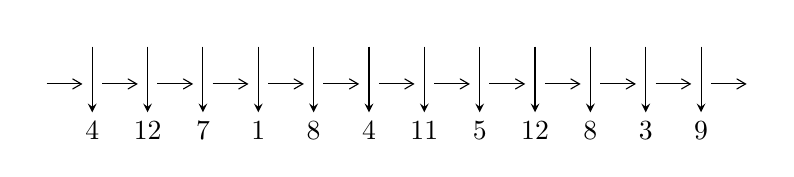
\begin{tikzpicture}[x=20pt, y=17pt]
	% nodes
	\node (C0) at (0, 0) {};
	\node (C1) at (1, 0) {};
	\node (C1U) at (1, +1) {};
	\node (C1D) at (1, -1) {4};

	\node (C2) at (2, 0) {};
	\node (C2U) at (2, +1) {};
	\node (C2D) at (2, -1) {12};

	\node (C3) at (3, 0) {};
	\node (C3U) at (3, +1) {};
	\node (C3D) at (3, -1) {7};

	\node (C4) at (4, 0) {};
	\node (C4U) at (4, +1) {};
	\node (C4D) at (4, -1) {1};

	\node (C5) at (5, 0) {};
	\node (C5U) at (5, +1) {};
	\node (C5D) at (5, -1) {8};

	\node (C6) at (6, 0) {};
	\node (C6U) at (6, +1) {};
	\node (C6D) at (6, -1) {4};

	\node (C7) at (7, 0) {};
	\node (C7U) at (7, +1) {};
	\node (C7D) at (7, -1) {11};

	\node (C8) at (8, 0) {};
	\node (C8U) at (8, +1) {};
	\node (C8D) at (8, -1) {5};

	\node (C9) at (9, 0) {};
	\node (C9U) at (9, +1) {};
	\node (C9D) at (9, -1) {12};

	\node (C10) at (10, 0) {};
	\node (C10U) at (10, +1) {};
	\node (C10D) at (10, -1) {8};

	\node (C11) at (11, 0) {};
	\node (C11U) at (11, +1) {};
	\node (C11D) at (11, -1) {3};

	\node (C12) at (12, 0) {};
	\node (C12U) at (12, +1) {};
	\node (C12D) at (12, -1) {9};
	\node (C13) at (13, 0) {};

	% arrows
	\draw[->,>={angle 60}]
	(C0) edge (C1) (C1) edge (C2) (C2) edge (C3) (C3) edge (C4) (C4) edge (C5) (C5) edge (C6) (C6) edge (C7) (C7) edge (C8) (C8) edge (C9) (C9) edge (C10) (C10) edge (C11) (C11) edge (C12) (C12) edge (C13) ;	\draw[->,>=stealth]
	(C1U) edge (C1D) (C2U) edge (C2D) (C3U) edge (C3D) (C4U) edge (C4D) (C5U) edge (C5D) (C6U) edge (C6D) (C7U) edge (C7D) (C8U) edge (C8D) (C9U) edge (C9D) (C10U) edge (C10D) (C11U) edge (C11D) (C12U) edge (C12D) ;
	\end{tikzpicture} \\
\hhline{~~} \\& 
\textbf{Solving Sequence} \\ \cline{2-2} 
 &
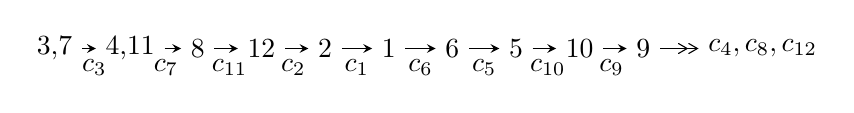
\begin{tikzpicture}[x=23pt, y=7pt]
	% node
	\node (A0) at (-1/8, 0) {3,7};
	\node (A1) at (17/16, 0) {4,11};
	\node (A2) at (17/8, 0) {8};
	\node (A3) at (25/8, 0) {12};
	\node (A4) at (33/8, 0) {2};
	\node (A5) at (41/8, 0) {1};
	\node (A6) at (49/8, 0) {6};
	\node (A7) at (57/8, 0) {5};
	\node (A8) at (65/8, 0) {10};
	\node (A9) at (73/8, 0) {9};
	\node (C1) at (1/2, -1) {$c_{3}$};
	\node (C2) at (13/8, -1) {$c_{7}$};
	\node (C3) at (21/8, -1) {$c_{11}$};
	\node (C4) at (29/8, -1) {$c_{2}$};
	\node (C5) at (37/8, -1) {$c_{1}$};
	\node (C6) at (45/8, -1) {$c_{6}$};
	\node (C7) at (53/8, -1) {$c_{5}$};
	\node (C8) at (61/8, -1) {$c_{10}$};
	\node (C9) at (69/8, -1) {$c_{9}$};
	\node (A10) at (11, 0) {$c_{4},c_{8},c_{12}$};

	% edge
	\draw[->,>=stealth]	
	(A0) edge (A1) (A1) edge (A2) (A2) edge (A3) (A3) edge (A4) (A4) edge (A5) (A5) edge (A6) (A6) edge (A7) (A7) edge (A8) (A8) edge (A9) ;
	\draw[->>,>={angle 60}]	
	(A9) edge (A10);
\end{tikzpicture} \\ 

\end{tabular} \\

\footnotetext{
The image of knot diagram is generated by the software ``\textbf{Draw programme}" developed by Andrew Bartholomew(\url{http://www.layer8.co.uk/maths/draw/index.htm\#Running-draw}), where we modified some parts for our purpose(\url{https://github.com/CATsTAILs/LinksPainter}).
}\phantom \\ \newline 
\centering \textbf{Ideals for irreducible components\footnotemark of $X_{\text{par}}$} 
 
\begin{align*}
I^u_{1}&=\langle 
b- u,\;a+1,\;u^3+u^2+2 u-1\rangle \\
I^u_{2}&=\langle 
b- u,\;-2 u^{15}+4 u^{14}+\cdots+2 a+5,\\
\phantom{I^u_{2}}&\phantom{= \langle  }u^{16}- u^{15}+6 u^{14}-3 u^{13}+17 u^{12}-5 u^{11}+30 u^{10}-4 u^9+33 u^8-3 u^7+22 u^6-4 u^5+8 u^4-5 u^3+3 u^2-3 u+1\rangle \\
I^u_{3}&=\langle 
-2 u^{15}-8 u^{13}-5 u^{12}-20 u^{11}-14 u^{10}-28 u^9-24 u^8-22 u^7-14 u^6- u^4+6 u^3+2 u^2+2 b+u-2,\;a+1,\\
\phantom{I^u_{3}}&\phantom{= \langle  }u^{16}- u^{15}+6 u^{14}-3 u^{13}+17 u^{12}-5 u^{11}+30 u^{10}-4 u^9+33 u^8-3 u^7+22 u^6-4 u^5+8 u^4-5 u^3+3 u^2-3 u+1\rangle \\
I^u_{4}&=\langle 
14971 u^{15}+114227 u^{14}+\cdots+20848 b+188080,\;11755 u^{15}+75853 u^{14}+\cdots+41696 a-119840,\\
\phantom{I^u_{4}}&\phantom{= \langle  }u^{16}+9 u^{15}+\cdots+64 u+32\rangle \\
I^u_{5}&=\langle 
b+u,\;a+1,\;u^4+u^2+2 u+1\rangle \\
I^u_{6}&=\langle 
b-2 u-1,\;a+1,\;u^2+u+1\rangle \\
I^u_{7}&=\langle 
b+u,\;a+u-1,\;u^2+u+1\rangle \\
I^u_{8}&=\langle 
2 b- u-1,\;6 a+u-3,\;u^2+3\rangle \\
I^u_{9}&=\langle 
b+1,\;a+1,\;u^2- u+1\rangle \\
I^u_{10}&=\langle 
b- u,\;a+u-1,\;u^2- u+1\rangle \\
\end{align*}\\
\begin{align*}
I^u_{11}&=\langle 
b- a,\;a^2- a+1,\;u+1\rangle \\
I^u_{12}&=\langle 
u^3- a u- u^2+b+3 u-2,\;2 u^4 a-2 u^3 a+7 u^2 a+u^3+a^2-5 a u+3 a+3 u,\;u^5- u^4+4 u^3-3 u^2+3 u-1\rangle \\
I^u_{13}&=\langle 
u^8-2 u^7+2 u^6-4 u^5+6 u^4-3 u^3+4 u^2+2 b-3 u,\\
\phantom{I^u_{13}}&\phantom{= \langle  }-2 u^9+3 u^8-4 u^7+10 u^6-12 u^5+10 u^4-17 u^3+10 u^2+2 a-9 u+4,\\
\phantom{I^u_{13}}&\phantom{= \langle  }u^{10}-2 u^9+3 u^8-6 u^7+8 u^6-8 u^5+11 u^4-8 u^3+7 u^2-4 u+1\rangle \\
I^u_{14}&=\langle 
u^9-2 u^8+2 u^7-4 u^6+6 u^5-5 u^4+6 u^3-5 u^2+2 b+4 u-2,\\
\phantom{I^u_{14}}&\phantom{= \langle  }- u^7+2 u^6-2 u^5+4 u^4-6 u^3+3 u^2+2 a-4 u+3,\\
\phantom{I^u_{14}}&\phantom{= \langle  }u^{10}-2 u^9+3 u^8-6 u^7+8 u^6-8 u^5+11 u^4-8 u^3+7 u^2-4 u+1\rangle \\
I^u_{15}&=\langle 
b+u,\;a+1,\;u^3- u^2+2 u-1\rangle \\
I^u_{16}&=\langle 
b+u,\;2 u^5+5 u^3-3 u^2+a+3 u-2,\;u^6- u^5+3 u^4-4 u^3+4 u^2-3 u+1\rangle \\
I^u_{17}&=\langle 
- u^5+u^4+b- u,\;- u^4+u^3+a-1,\;u^6-2 u^5+2 u^4-2 u^3+2 u^2- u+1\rangle \\
I^u_{18}&=\langle 
2 u^5- u^4+5 u^3-5 u^2+b+4 u-2,\;a+1,\;u^6- u^5+3 u^4-4 u^3+4 u^2-3 u+1\rangle \\
I^u_{19}&=\langle 
b- u,\;a+1,\;u^4+2 u^3+3 u^2+2 u+1\rangle \\
\\
\end{align*}
\raggedright * 19 irreducible components of $\dim_{\mathbb{C}}=0$, with total 122 representations.\\
\footnotetext{All coefficients of polynomials are rational numbers. But the coefficients are sometimes approximated in decimal forms when there is not enough margin.}
\newpage
\renewcommand{\arraystretch}{1}
\centering \section*{I. $I^u_{1}= \langle b- u,\;a+1,\;u^3+u^2+2 u-1 \rangle$}
\flushleft \textbf{(i) Arc colorings}\\
\begin{tabular}{m{7pt} m{180pt} m{7pt} m{180pt} }
\flushright $a_{3}=$&$\begin{pmatrix}1\\0\end{pmatrix}$ \\
\flushright $a_{7}=$&$\begin{pmatrix}0\\u\end{pmatrix}$ \\
\flushright $a_{4}=$&$\begin{pmatrix}1\\u^2\end{pmatrix}$ \\
\flushright $a_{11}=$&$\begin{pmatrix}-1\\u\end{pmatrix}$ \\
\flushright $a_{8}=$&$\begin{pmatrix}- u\\u^2+u\end{pmatrix}$ \\
\flushright $a_{12}=$&$\begin{pmatrix}- u-1\\u\end{pmatrix}$ \\
\flushright $a_{2}=$&$\begin{pmatrix}u^2+u+1\\- u^2\end{pmatrix}$ \\
\flushright $a_{1}=$&$\begin{pmatrix}u^2+1\\2 u-1\end{pmatrix}$ \\
\flushright $a_{6}=$&$\begin{pmatrix}u\\- u^2- u+1\end{pmatrix}$ \\
\flushright $a_{5}=$&$\begin{pmatrix}u^2+u\\- u^2+u\end{pmatrix}$ \\
\flushright $a_{10}=$&$\begin{pmatrix}- u^2-1\\- u+1\end{pmatrix}$ \\
\flushright $a_{9}=$&$\begin{pmatrix}u-1\\- u^2- u+1\end{pmatrix}$\\&\end{tabular}
\flushleft \textbf{(ii) Obstruction class $= -1$}\\~\\
\flushleft \textbf{(iii) Cusp Shapes $= -6 u-9$}\\~\\
\newpage\renewcommand{\arraystretch}{1}
\flushleft \textbf{(iv) u-Polynomials at the component}\newline \\
\begin{tabular}{m{50pt}|m{274pt}}
Crossings & \hspace{64pt}u-Polynomials at each crossing \\
\hline $$\begin{aligned}c_{1},c_{2},c_{3}\\c_{4},c_{5},c_{6}\\c_{7},c_{8},c_{9}\\c_{10},c_{11},c_{12}\end{aligned}$$&$\begin{aligned}
&u^3- u^2+2 u+1
\end{aligned}$\\
\hline
\end{tabular}\\~\\
\newpage\renewcommand{\arraystretch}{1}
\flushleft \textbf{(v) Riley Polynomials at the component}\newline \\
\begin{tabular}{m{50pt}|m{274pt}}
Crossings & \hspace{64pt}Riley Polynomials at each crossing \\
\hline $$\begin{aligned}c_{1},c_{2},c_{3}\\c_{4},c_{5},c_{6}\\c_{7},c_{8},c_{9}\\c_{10},c_{11},c_{12}\end{aligned}$$&$\begin{aligned}
&y^3+3 y^2+6 y-1
\end{aligned}$\\
\hline
\end{tabular}\\~\\
\newpage\flushleft \textbf{(vi) Complex Volumes and Cusp Shapes}
$$\begin{array}{c|c|c}  
\text{Solutions to }I^u_{1}& \I (\text{vol} + \sqrt{-1}CS) & \text{Cusp shape}\\
 \hline 
\begin{aligned}
u &= -0.69632 + 1.43595 I \\
a &= -1.00000\phantom{ +0.000000I} \\
b &= -0.69632 + 1.43595 I\end{aligned}
 & \phantom{-}8.6715 + 17.0103 I & -4.82206 - 8.61570 I \\ \hline\begin{aligned}
u &= -0.69632 - 1.43595 I \\
a &= -1.00000\phantom{ +0.000000I} \\
b &= -0.69632 - 1.43595 I\end{aligned}
 & \phantom{-}8.6715 - 17.0103 I & -4.82206 + 8.61570 I \\ \hline\begin{aligned}
u &= \phantom{-}0.392647\phantom{ +0.000000I} \\
a &= -1.00000\phantom{ +0.000000I} \\
b &= \phantom{-}0.392647\phantom{ +0.000000I}\end{aligned}
 & -0.893590\phantom{ +0.000000I} & -11.3560\phantom{ +0.000000I}\\
 \hline 
 \end{array}$$\newpage\newpage\renewcommand{\arraystretch}{1}
\centering \section*{II. $I^u_{2}= \langle b- u,\;-2 u^{15}+4 u^{14}+\cdots+2 a+5,\;u^{16}- u^{15}+\cdots-3 u+1 \rangle$}
\flushleft \textbf{(i) Arc colorings}\\
\begin{tabular}{m{7pt} m{180pt} m{7pt} m{180pt} }
\flushright $a_{3}=$&$\begin{pmatrix}1\\0\end{pmatrix}$ \\
\flushright $a_{7}=$&$\begin{pmatrix}0\\u\end{pmatrix}$ \\
\flushright $a_{4}=$&$\begin{pmatrix}1\\u^2\end{pmatrix}$ \\
\flushright $a_{11}=$&$\begin{pmatrix}u^{15}-2 u^{14}+\cdots+4 u-\frac{5}{2}\\u\end{pmatrix}$ \\
\flushright $a_{8}=$&$\begin{pmatrix}u^{15}+2 u^{14}+\cdots-5 u+2\\u^{15}-2 u^{14}+\cdots+5 u-1\end{pmatrix}$ \\
\flushright $a_{12}=$&$\begin{pmatrix}u^{15}-2 u^{14}+\cdots+3 u-\frac{5}{2}\\u\end{pmatrix}$ \\
\flushright $a_{2}=$&$\begin{pmatrix}u^{15}+4 u^{13}+\cdots-\frac{1}{2} u+2\\- u^2\end{pmatrix}$ \\
\flushright $a_{1}=$&$\begin{pmatrix}2 u^{15}+\frac{1}{2} u^{14}+\cdots-\frac{5}{2} u+3\\-\frac{1}{2} u^{15}- u^{14}+\cdots+\frac{7}{2} u-\frac{3}{2}\end{pmatrix}$ \\
\flushright $a_{6}=$&$\begin{pmatrix}u\\u^3+u\end{pmatrix}$ \\
\flushright $a_{5}=$&$\begin{pmatrix}-\frac{1}{2} u^{15}+\frac{5}{2} u^{14}+\cdots-\frac{9}{2} u+2\\u^{15}- u^{14}+\cdots+\frac{5}{2} u-\frac{1}{2}\end{pmatrix}$ \\
\flushright $a_{10}=$&$\begin{pmatrix}-\frac{3}{2} u^{15}-6 u^{13}+\cdots+u-\frac{5}{2}\\\frac{1}{2} u^{15}+u^{14}+\cdots-3 u+2\end{pmatrix}$ \\
\flushright $a_{9}=$&$\begin{pmatrix}-\frac{3}{2} u^{15}+2 u^{14}+\cdots-5 u+\frac{1}{2}\\u^{15}-\frac{1}{2} u^{14}+\cdots+u+\frac{1}{2}\end{pmatrix}$\\&\end{tabular}
\flushleft \textbf{(ii) Obstruction class $= -1$}\\~\\
\flushleft \textbf{(iii) Cusp Shapes $= 3 u^{15}+14 u^{13}+8 u^{12}+38 u^{11}+28 u^{10}+64 u^9+54 u^8+68 u^7+48 u^6+35 u^5+12 u^4+2 u^3-10 u^2-5 u-8$}\\~\\
\newpage\renewcommand{\arraystretch}{1}
\flushleft \textbf{(iv) u-Polynomials at the component}\newline \\
\begin{tabular}{m{50pt}|m{274pt}}
Crossings & \hspace{64pt}u-Polynomials at each crossing \\
\hline $$\begin{aligned}c_{1},c_{4},c_{7}\\c_{10}\end{aligned}$$&$\begin{aligned}
&u^{16}-9 u^{15}+\cdots-64 u+32
\end{aligned}$\\
\hline $$\begin{aligned}c_{2},c_{3},c_{5}\\c_{6},c_{8},c_{9}\\c_{11},c_{12}\end{aligned}$$&$\begin{aligned}
&u^{16}+u^{15}+\cdots+3 u+1
\end{aligned}$\\
\hline
\end{tabular}\\~\\
\newpage\renewcommand{\arraystretch}{1}
\flushleft \textbf{(v) Riley Polynomials at the component}\newline \\
\begin{tabular}{m{50pt}|m{274pt}}
Crossings & \hspace{64pt}Riley Polynomials at each crossing \\
\hline $$\begin{aligned}c_{1},c_{4},c_{7}\\c_{10}\end{aligned}$$&$\begin{aligned}
&y^{16}+11 y^{15}+\cdots-2560 y+1024
\end{aligned}$\\
\hline $$\begin{aligned}c_{2},c_{3},c_{5}\\c_{6},c_{8},c_{9}\\c_{11},c_{12}\end{aligned}$$&$\begin{aligned}
&y^{16}+11 y^{15}+\cdots-3 y+1
\end{aligned}$\\
\hline
\end{tabular}\\~\\
\newpage\flushleft \textbf{(vi) Complex Volumes and Cusp Shapes}
$$\begin{array}{c|c|c}  
\text{Solutions to }I^u_{2}& \I (\text{vol} + \sqrt{-1}CS) & \text{Cusp shape}\\
 \hline 
\begin{aligned}
u &= \phantom{-}0.155071 + 0.982491 I \\
a &= \phantom{-}1.85344 - 0.16488 I \\
b &= \phantom{-}0.155071 + 0.982491 I\end{aligned}
 & \phantom{-}11.07300 + 2.11324 I & -4.13579 - 3.29911 I \\ \hline\begin{aligned}
u &= \phantom{-}0.155071 - 0.982491 I \\
a &= \phantom{-}1.85344 + 0.16488 I \\
b &= \phantom{-}0.155071 - 0.982491 I\end{aligned}
 & \phantom{-}11.07300 - 2.11324 I & -4.13579 + 3.29911 I \\ \hline\begin{aligned}
u &= \phantom{-}0.263127 + 0.911584 I \\
a &= -0.593560 - 1.154310 I \\
b &= \phantom{-}0.263127 + 0.911584 I\end{aligned}
 & \phantom{-}1.97235\phantom{ +0.000000I} & -2.75019 + 0. I\phantom{ +0.000000I} \\ \hline\begin{aligned}
u &= \phantom{-}0.263127 - 0.911584 I \\
a &= -0.593560 + 1.154310 I \\
b &= \phantom{-}0.263127 - 0.911584 I\end{aligned}
 & \phantom{-}1.97235\phantom{ +0.000000I} & -2.75019 + 0. I\phantom{ +0.000000I} \\ \hline\begin{aligned}
u &= -0.415478 + 1.074820 I \\
a &= -0.325650 - 1.226660 I \\
b &= -0.415478 + 1.074820 I\end{aligned}
 & \phantom{-}4.56396 + 9.62189 I & -5.35347 - 7.22561 I \\ \hline\begin{aligned}
u &= -0.415478 - 1.074820 I \\
a &= -0.325650 + 1.226660 I \\
b &= -0.415478 - 1.074820 I\end{aligned}
 & \phantom{-}4.56396 - 9.62189 I & -5.35347 + 7.22561 I \\ \hline\begin{aligned}
u &= -0.635797 + 0.475943 I \\
a &= -0.30659 - 1.45911 I \\
b &= -0.635797 + 0.475943 I\end{aligned}
 & \phantom{-}2.73466 - 5.62392 I & -7.83043 + 1.63381 I \\ \hline\begin{aligned}
u &= -0.635797 - 0.475943 I \\
a &= -0.30659 + 1.45911 I \\
b &= -0.635797 - 0.475943 I\end{aligned}
 & \phantom{-}2.73466 + 5.62392 I & -7.83043 - 1.63381 I \\ \hline\begin{aligned}
u &= -0.640425 + 1.031810 I \\
a &= -1.163390 + 0.606464 I \\
b &= -0.640425 + 1.031810 I\end{aligned}
 & \phantom{-}11.07300 + 2.11324 I & -4.13579 - 3.29911 I \\ \hline\begin{aligned}
u &= -0.640425 - 1.031810 I \\
a &= -1.163390 - 0.606464 I \\
b &= -0.640425 - 1.031810 I\end{aligned}
 & \phantom{-}11.07300 - 2.11324 I & -4.13579 + 3.29911 I\\
 \hline 
 \end{array}$$\newpage$$\begin{array}{c|c|c}  
\text{Solutions to }I^u_{2}& \I (\text{vol} + \sqrt{-1}CS) & \text{Cusp shape}\\
 \hline 
\begin{aligned}
u &= \phantom{-}0.59989 + 1.32302 I \\
a &= \phantom{-}0.816913 - 0.091000 I \\
b &= \phantom{-}0.59989 + 1.32302 I\end{aligned}
 & \phantom{-}2.73466 - 5.62392 I & -7.83043 + 1.63381 I \\ \hline\begin{aligned}
u &= \phantom{-}0.59989 - 1.32302 I \\
a &= \phantom{-}0.816913 + 0.091000 I \\
b &= \phantom{-}0.59989 - 1.32302 I\end{aligned}
 & \phantom{-}2.73466 + 5.62392 I & -7.83043 - 1.63381 I \\ \hline\begin{aligned}
u &= \phantom{-}0.75412 + 1.29455 I \\
a &= \phantom{-}0.993241 + 0.183480 I \\
b &= \phantom{-}0.75412 + 1.29455 I\end{aligned}
 & \phantom{-}4.56396 - 9.62189 I & -5.35347 + 7.22561 I \\ \hline\begin{aligned}
u &= \phantom{-}0.75412 - 1.29455 I \\
a &= \phantom{-}0.993241 - 0.183480 I \\
b &= \phantom{-}0.75412 - 1.29455 I\end{aligned}
 & \phantom{-}4.56396 + 9.62189 I & -5.35347 - 7.22561 I \\ \hline\begin{aligned}
u &= \phantom{-}0.419493 + 0.126250 I \\
a &= -0.774408 + 0.831625 I \\
b &= \phantom{-}0.419493 + 0.126250 I\end{aligned}
 & -0.882161\phantom{ +0.000000I} & -11.61043 + 0. I\phantom{ +0.000000I} \\ \hline\begin{aligned}
u &= \phantom{-}0.419493 - 0.126250 I \\
a &= -0.774408 - 0.831625 I \\
b &= \phantom{-}0.419493 - 0.126250 I\end{aligned}
 & -0.882161\phantom{ +0.000000I} & -11.61043 + 0. I\phantom{ +0.000000I}\\
 \hline 
 \end{array}$$\newpage\newpage\renewcommand{\arraystretch}{1}
\centering \section*{III. $I^u_{3}= \langle -2 u^{15}-8 u^{13}+\cdots+2 b-2,\;a+1,\;u^{16}- u^{15}+\cdots-3 u+1 \rangle$}
\flushleft \textbf{(i) Arc colorings}\\
\begin{tabular}{m{7pt} m{180pt} m{7pt} m{180pt} }
\flushright $a_{3}=$&$\begin{pmatrix}1\\0\end{pmatrix}$ \\
\flushright $a_{7}=$&$\begin{pmatrix}0\\u\end{pmatrix}$ \\
\flushright $a_{4}=$&$\begin{pmatrix}1\\u^2\end{pmatrix}$ \\
\flushright $a_{11}=$&$\begin{pmatrix}-1\\u^{15}+4 u^{13}+\cdots-\frac{1}{2} u+1\end{pmatrix}$ \\
\flushright $a_{8}=$&$\begin{pmatrix}- u\\u^{15}-2 u^{14}+\cdots+5 u-1\end{pmatrix}$ \\
\flushright $a_{12}=$&$\begin{pmatrix}- u^{15}-4 u^{13}+\cdots+\frac{1}{2} u-2\\u^{15}+4 u^{13}+\cdots-\frac{1}{2} u+1\end{pmatrix}$ \\
\flushright $a_{2}=$&$\begin{pmatrix}-2 u^{15}+\frac{5}{2} u^{14}+\cdots-\frac{11}{2} u+3\\3 u^{15}-\frac{5}{2} u^{14}+\cdots+5 u-1\end{pmatrix}$ \\
\flushright $a_{1}=$&$\begin{pmatrix}-\frac{1}{2} u^{15}+\frac{3}{2} u^{14}+\cdots-4 u+\frac{5}{2}\\2 u^{15}-\frac{5}{2} u^{14}+\cdots+5 u-\frac{3}{2}\end{pmatrix}$ \\
\flushright $a_{6}=$&$\begin{pmatrix}u\\u^3+u\end{pmatrix}$ \\
\flushright $a_{5}=$&$\begin{pmatrix}-\frac{3}{2} u^{15}+2 u^{14}+\cdots-3 u+1\\\frac{3}{2} u^{15}- u^{14}+\cdots-4 u^2+2 u\end{pmatrix}$ \\
\flushright $a_{10}=$&$\begin{pmatrix}- u^2-1\\-\frac{1}{2} u^{14}-\frac{5}{2} u^{12}+\cdots+u^2+\frac{3}{2} u\end{pmatrix}$ \\
\flushright $a_{9}=$&$\begin{pmatrix}-\frac{1}{2} u^{15}-\frac{1}{2} u^{14}+\cdots+\frac{3}{2} u-1\\- u^{15}+u^{14}+\cdots-\frac{3}{2} u+\frac{1}{2}\end{pmatrix}$\\&\end{tabular}
\flushleft \textbf{(ii) Obstruction class $= -1$}\\~\\
\flushleft \textbf{(iii) Cusp Shapes $= 3 u^{15}+14 u^{13}+8 u^{12}+38 u^{11}+28 u^{10}+64 u^9+54 u^8+68 u^7+48 u^6+35 u^5+12 u^4+2 u^3-10 u^2-5 u-8$}\\~\\
\newpage\renewcommand{\arraystretch}{1}
\flushleft \textbf{(iv) u-Polynomials at the component}\newline \\
\begin{tabular}{m{50pt}|m{274pt}}
Crossings & \hspace{64pt}u-Polynomials at each crossing \\
\hline $$\begin{aligned}c_{1},c_{3},c_{4}\\c_{6},c_{7},c_{9}\\c_{10},c_{12}\end{aligned}$$&$\begin{aligned}
&u^{16}+u^{15}+\cdots+3 u+1
\end{aligned}$\\
\hline $$\begin{aligned}c_{2},c_{5},c_{8}\\c_{11}\end{aligned}$$&$\begin{aligned}
&u^{16}-9 u^{15}+\cdots-64 u+32
\end{aligned}$\\
\hline
\end{tabular}\\~\\
\newpage\renewcommand{\arraystretch}{1}
\flushleft \textbf{(v) Riley Polynomials at the component}\newline \\
\begin{tabular}{m{50pt}|m{274pt}}
Crossings & \hspace{64pt}Riley Polynomials at each crossing \\
\hline $$\begin{aligned}c_{1},c_{3},c_{4}\\c_{6},c_{7},c_{9}\\c_{10},c_{12}\end{aligned}$$&$\begin{aligned}
&y^{16}+11 y^{15}+\cdots-3 y+1
\end{aligned}$\\
\hline $$\begin{aligned}c_{2},c_{5},c_{8}\\c_{11}\end{aligned}$$&$\begin{aligned}
&y^{16}+11 y^{15}+\cdots-2560 y+1024
\end{aligned}$\\
\hline
\end{tabular}\\~\\
\newpage\flushleft \textbf{(vi) Complex Volumes and Cusp Shapes}
$$\begin{array}{c|c|c}  
\text{Solutions to }I^u_{3}& \I (\text{vol} + \sqrt{-1}CS) & \text{Cusp shape}\\
 \hline 
\begin{aligned}
u &= \phantom{-}0.155071 + 0.982491 I \\
a &= -1.00000\phantom{ +0.000000I} \\
b &= -0.44941 - 1.79542 I\end{aligned}
 & \phantom{-}11.07300 + 2.11324 I & -4.13579 - 3.29911 I \\ \hline\begin{aligned}
u &= \phantom{-}0.155071 - 0.982491 I \\
a &= -1.00000\phantom{ +0.000000I} \\
b &= -0.44941 + 1.79542 I\end{aligned}
 & \phantom{-}11.07300 - 2.11324 I & -4.13579 + 3.29911 I \\ \hline\begin{aligned}
u &= \phantom{-}0.263127 + 0.911584 I \\
a &= -1.00000\phantom{ +0.000000I} \\
b &= -0.896070 + 0.844811 I\end{aligned}
 & \phantom{-}1.97235\phantom{ +0.000000I} & -2.75019 + 0. I\phantom{ +0.000000I} \\ \hline\begin{aligned}
u &= \phantom{-}0.263127 - 0.911584 I \\
a &= -1.00000\phantom{ +0.000000I} \\
b &= -0.896070 - 0.844811 I\end{aligned}
 & \phantom{-}1.97235\phantom{ +0.000000I} & -2.75019 + 0. I\phantom{ +0.000000I} \\ \hline\begin{aligned}
u &= -0.415478 + 1.074820 I \\
a &= -1.00000\phantom{ +0.000000I} \\
b &= -1.45373 - 0.15964 I\end{aligned}
 & \phantom{-}4.56396 + 9.62189 I & -5.35347 - 7.22561 I \\ \hline\begin{aligned}
u &= -0.415478 - 1.074820 I \\
a &= -1.00000\phantom{ +0.000000I} \\
b &= -1.45373 + 0.15964 I\end{aligned}
 & \phantom{-}4.56396 - 9.62189 I & -5.35347 + 7.22561 I \\ \hline\begin{aligned}
u &= -0.635797 + 0.475943 I \\
a &= -1.00000\phantom{ +0.000000I} \\
b &= -0.889379 - 0.781779 I\end{aligned}
 & \phantom{-}2.73466 - 5.62392 I & -7.83043 + 1.63381 I \\ \hline\begin{aligned}
u &= -0.635797 - 0.475943 I \\
a &= -1.00000\phantom{ +0.000000I} \\
b &= -0.889379 + 0.781779 I\end{aligned}
 & \phantom{-}2.73466 + 5.62392 I & -7.83043 - 1.63381 I \\ \hline\begin{aligned}
u &= -0.640425 + 1.031810 I \\
a &= -1.00000\phantom{ +0.000000I} \\
b &= -0.11931 + 1.58879 I\end{aligned}
 & \phantom{-}11.07300 + 2.11324 I & -4.13579 - 3.29911 I \\ \hline\begin{aligned}
u &= -0.640425 - 1.031810 I \\
a &= -1.00000\phantom{ +0.000000I} \\
b &= -0.11931 - 1.58879 I\end{aligned}
 & \phantom{-}11.07300 - 2.11324 I & -4.13579 + 3.29911 I\\
 \hline 
 \end{array}$$\newpage$$\begin{array}{c|c|c}  
\text{Solutions to }I^u_{3}& \I (\text{vol} + \sqrt{-1}CS) & \text{Cusp shape}\\
 \hline 
\begin{aligned}
u &= \phantom{-}0.59989 + 1.32302 I \\
a &= -1.00000\phantom{ +0.000000I} \\
b &= -0.610454 - 1.026200 I\end{aligned}
 & \phantom{-}2.73466 - 5.62392 I & -7.83043 + 1.63381 I \\ \hline\begin{aligned}
u &= \phantom{-}0.59989 - 1.32302 I \\
a &= -1.00000\phantom{ +0.000000I} \\
b &= -0.610454 + 1.026200 I\end{aligned}
 & \phantom{-}2.73466 + 5.62392 I & -7.83043 - 1.63381 I \\ \hline\begin{aligned}
u &= \phantom{-}0.75412 + 1.29455 I \\
a &= -1.00000\phantom{ +0.000000I} \\
b &= -0.51150 - 1.42416 I\end{aligned}
 & \phantom{-}4.56396 - 9.62189 I & -5.35347 + 7.22561 I \\ \hline\begin{aligned}
u &= \phantom{-}0.75412 - 1.29455 I \\
a &= -1.00000\phantom{ +0.000000I} \\
b &= -0.51150 + 1.42416 I\end{aligned}
 & \phantom{-}4.56396 + 9.62189 I & -5.35347 - 7.22561 I \\ \hline\begin{aligned}
u &= \phantom{-}0.419493 + 0.126250 I \\
a &= -1.00000\phantom{ +0.000000I} \\
b &= \phantom{-}0.429851 - 0.251093 I\end{aligned}
 & -0.882161\phantom{ +0.000000I} & -11.61043 + 0. I\phantom{ +0.000000I} \\ \hline\begin{aligned}
u &= \phantom{-}0.419493 - 0.126250 I \\
a &= -1.00000\phantom{ +0.000000I} \\
b &= \phantom{-}0.429851 + 0.251093 I\end{aligned}
 & -0.882161\phantom{ +0.000000I} & -11.61043 + 0. I\phantom{ +0.000000I}\\
 \hline 
 \end{array}$$\newpage\newpage\renewcommand{\arraystretch}{1}
\centering \section*{IV. $I^u_{4}= \langle 14971 u^{15}+114227 u^{14}+\cdots+20848 b+188080,\;11755 u^{15}+75853 u^{14}+\cdots+41696 a-119840,\;u^{16}+9 u^{15}+\cdots+64 u+32 \rangle$}
\flushleft \textbf{(i) Arc colorings}\\
\begin{tabular}{m{7pt} m{180pt} m{7pt} m{180pt} }
\flushright $a_{3}=$&$\begin{pmatrix}1\\0\end{pmatrix}$ \\
\flushright $a_{7}=$&$\begin{pmatrix}0\\u\end{pmatrix}$ \\
\flushright $a_{4}=$&$\begin{pmatrix}1\\u^2\end{pmatrix}$ \\
\flushright $a_{11}=$&$\begin{pmatrix}-0.281922 u^{15}-1.81919 u^{14}+\cdots-4.33596 u+2.87414\\-0.718102 u^{15}-5.47904 u^{14}+\cdots-20.9171 u-9.02149\end{pmatrix}$ \\
\flushright $a_{8}=$&$\begin{pmatrix}0.706255 u^{15}+5.65340 u^{14}+\cdots+24.6506 u+9.22947\\0.702897 u^{15}+6.15119 u^{14}+\cdots+36.9708 u+22.6002\end{pmatrix}$ \\
\flushright $a_{12}=$&$\begin{pmatrix}0.436181 u^{15}+3.65985 u^{14}+\cdots+16.5812 u+11.8956\\-0.718102 u^{15}-5.47904 u^{14}+\cdots-20.9171 u-9.02149\end{pmatrix}$ \\
\flushright $a_{2}=$&$\begin{pmatrix}-0.00335764 u^{15}+0.497794 u^{14}+\cdots+11.3202 u+14.3707\\-0.702897 u^{15}-6.15119 u^{14}+\cdots-35.9708 u-22.6002\end{pmatrix}$ \\
\flushright $a_{1}=$&$\begin{pmatrix}0.0881619 u^{15}+0.918649 u^{14}+\cdots+9.03473 u+8.66692\\-0.149367 u^{15}-1.50173 u^{14}+\cdots-13.1190 u-9.70990\end{pmatrix}$ \\
\flushright $a_{6}=$&$\begin{pmatrix}u\\u^3+u\end{pmatrix}$ \\
\flushright $a_{5}=$&$\begin{pmatrix}-0.321901 u^{15}-3.03118 u^{14}+\cdots-19.7034 u-16.2621\\-0.268755 u^{15}-2.46590 u^{14}+\cdots-14.9006 u-13.2295\end{pmatrix}$ \\
\flushright $a_{10}=$&$\begin{pmatrix}0.141045 u^{15}+1.82840 u^{14}+\cdots+17.8037 u+16.0787\\0.424885 u^{15}+4.19350 u^{14}+\cdots+29.8853 u+27.4927\end{pmatrix}$ \\
\flushright $a_{9}=$&$\begin{pmatrix}0.333245 u^{15}+3.21899 u^{14}+\cdots+19.1554 u+15.4597\\0.333941 u^{15}+3.80516 u^{14}+\cdots+33.7444 u+30.7329\end{pmatrix}$\\&\end{tabular}
\flushleft \textbf{(ii) Obstruction class $= -1$}\\~\\
\flushleft \textbf{(iii) Cusp Shapes $= -\frac{16065}{5212} u^{15}-\frac{133039}{5212} u^{14}+\cdots-\frac{159664}{1303} u-\frac{98654}{1303}$}\\~\\
\newpage\renewcommand{\arraystretch}{1}
\flushleft \textbf{(iv) u-Polynomials at the component}\newline \\
\begin{tabular}{m{50pt}|m{274pt}}
Crossings & \hspace{64pt}u-Polynomials at each crossing \\
\hline $$\begin{aligned}c_{1},c_{2},c_{4}\\c_{5},c_{7},c_{8}\\c_{10},c_{11}\end{aligned}$$&$\begin{aligned}
&u^{16}+u^{15}+\cdots+3 u+1
\end{aligned}$\\
\hline $$\begin{aligned}c_{3},c_{6},c_{9}\\c_{12}\end{aligned}$$&$\begin{aligned}
&u^{16}-9 u^{15}+\cdots-64 u+32
\end{aligned}$\\
\hline
\end{tabular}\\~\\
\newpage\renewcommand{\arraystretch}{1}
\flushleft \textbf{(v) Riley Polynomials at the component}\newline \\
\begin{tabular}{m{50pt}|m{274pt}}
Crossings & \hspace{64pt}Riley Polynomials at each crossing \\
\hline $$\begin{aligned}c_{1},c_{2},c_{4}\\c_{5},c_{7},c_{8}\\c_{10},c_{11}\end{aligned}$$&$\begin{aligned}
&y^{16}+11 y^{15}+\cdots-3 y+1
\end{aligned}$\\
\hline $$\begin{aligned}c_{3},c_{6},c_{9}\\c_{12}\end{aligned}$$&$\begin{aligned}
&y^{16}+11 y^{15}+\cdots-2560 y+1024
\end{aligned}$\\
\hline
\end{tabular}\\~\\
\newpage\flushleft \textbf{(vi) Complex Volumes and Cusp Shapes}
$$\begin{array}{c|c|c}  
\text{Solutions to }I^u_{4}& \I (\text{vol} + \sqrt{-1}CS) & \text{Cusp shape}\\
 \hline 
\begin{aligned}
u &= -0.889379 + 0.781779 I \\
a &= -0.137916 - 0.656371 I \\
b &= -0.635797 - 0.475943 I\end{aligned}
 & \phantom{-}2.73466 + 5.62392 I & -7.83043 - 1.63381 I \\ \hline\begin{aligned}
u &= -0.889379 - 0.781779 I \\
a &= -0.137916 + 0.656371 I \\
b &= -0.635797 + 0.475943 I\end{aligned}
 & \phantom{-}2.73466 - 5.62392 I & -7.83043 + 1.63381 I \\ \hline\begin{aligned}
u &= -0.610454 + 1.026200 I \\
a &= \phantom{-}1.209120 - 0.134690 I \\
b &= \phantom{-}0.59989 - 1.32302 I\end{aligned}
 & \phantom{-}2.73466 + 5.62392 I & -7.83043 - 1.63381 I \\ \hline\begin{aligned}
u &= -0.610454 - 1.026200 I \\
a &= \phantom{-}1.209120 + 0.134690 I \\
b &= \phantom{-}0.59989 + 1.32302 I\end{aligned}
 & \phantom{-}2.73466 - 5.62392 I & -7.83043 + 1.63381 I \\ \hline\begin{aligned}
u &= -0.896070 + 0.844811 I \\
a &= -0.352314 + 0.685153 I \\
b &= \phantom{-}0.263127 + 0.911584 I\end{aligned}
 & \phantom{-}1.97235\phantom{ +0.000000I} & -2.75019 + 0. I\phantom{ +0.000000I} \\ \hline\begin{aligned}
u &= -0.896070 - 0.844811 I \\
a &= -0.352314 - 0.685153 I \\
b &= \phantom{-}0.263127 - 0.911584 I\end{aligned}
 & \phantom{-}1.97235\phantom{ +0.000000I} & -2.75019 + 0. I\phantom{ +0.000000I} \\ \hline\begin{aligned}
u &= -1.45373 + 0.15964 I \\
a &= -0.202173 - 0.761549 I \\
b &= -0.415478 - 1.074820 I\end{aligned}
 & \phantom{-}4.56396 - 9.62189 I & -5.35347 + 7.22561 I \\ \hline\begin{aligned}
u &= -1.45373 - 0.15964 I \\
a &= -0.202173 + 0.761549 I \\
b &= -0.415478 + 1.074820 I\end{aligned}
 & \phantom{-}4.56396 + 9.62189 I & -5.35347 - 7.22561 I \\ \hline\begin{aligned}
u &= \phantom{-}0.429851 + 0.251093 I \\
a &= -0.599708 + 0.644017 I \\
b &= \phantom{-}0.419493 - 0.126250 I\end{aligned}
 & -0.882161\phantom{ +0.000000I} & -11.61043 + 0. I\phantom{ +0.000000I} \\ \hline\begin{aligned}
u &= \phantom{-}0.429851 - 0.251093 I \\
a &= -0.599708 - 0.644017 I \\
b &= \phantom{-}0.419493 + 0.126250 I\end{aligned}
 & -0.882161\phantom{ +0.000000I} & -11.61043 + 0. I\phantom{ +0.000000I}\\
 \hline 
 \end{array}$$\newpage$$\begin{array}{c|c|c}  
\text{Solutions to }I^u_{4}& \I (\text{vol} + \sqrt{-1}CS) & \text{Cusp shape}\\
 \hline 
\begin{aligned}
u &= -0.51150 + 1.42416 I \\
a &= \phantom{-}0.973582 + 0.179848 I \\
b &= \phantom{-}0.75412 - 1.29455 I\end{aligned}
 & \phantom{-}4.56396 + 9.62189 I & -5.35347 - 7.22561 I \\ \hline\begin{aligned}
u &= -0.51150 - 1.42416 I \\
a &= \phantom{-}0.973582 - 0.179848 I \\
b &= \phantom{-}0.75412 + 1.29455 I\end{aligned}
 & \phantom{-}4.56396 - 9.62189 I & -5.35347 + 7.22561 I \\ \hline\begin{aligned}
u &= -0.11931 + 1.58879 I \\
a &= -0.675889 - 0.352334 I \\
b &= -0.640425 + 1.031810 I\end{aligned}
 & \phantom{-}11.07300 + 2.11324 I & -4.13579 - 3.29911 I \\ \hline\begin{aligned}
u &= -0.11931 - 1.58879 I \\
a &= -0.675889 + 0.352334 I \\
b &= -0.640425 - 1.031810 I\end{aligned}
 & \phantom{-}11.07300 - 2.11324 I & -4.13579 + 3.29911 I \\ \hline\begin{aligned}
u &= -0.44941 + 1.79542 I \\
a &= \phantom{-}0.535301 - 0.047620 I \\
b &= \phantom{-}0.155071 - 0.982491 I\end{aligned}
 & \phantom{-}11.07300 - 2.11324 I & -4.13579 + 3.29911 I \\ \hline\begin{aligned}
u &= -0.44941 - 1.79542 I \\
a &= \phantom{-}0.535301 + 0.047620 I \\
b &= \phantom{-}0.155071 + 0.982491 I\end{aligned}
 & \phantom{-}11.07300 + 2.11324 I & -4.13579 - 3.29911 I\\
 \hline 
 \end{array}$$\newpage\newpage\renewcommand{\arraystretch}{1}
\centering \section*{V. $I^u_{5}= \langle b+u,\;a+1,\;u^4+u^2+2 u+1 \rangle$}
\flushleft \textbf{(i) Arc colorings}\\
\begin{tabular}{m{7pt} m{180pt} m{7pt} m{180pt} }
\flushright $a_{3}=$&$\begin{pmatrix}1\\0\end{pmatrix}$ \\
\flushright $a_{7}=$&$\begin{pmatrix}0\\u\end{pmatrix}$ \\
\flushright $a_{4}=$&$\begin{pmatrix}1\\u^2\end{pmatrix}$ \\
\flushright $a_{11}=$&$\begin{pmatrix}-1\\- u\end{pmatrix}$ \\
\flushright $a_{8}=$&$\begin{pmatrix}- u\\- u^2+u\end{pmatrix}$ \\
\flushright $a_{12}=$&$\begin{pmatrix}u-1\\- u\end{pmatrix}$ \\
\flushright $a_{2}=$&$\begin{pmatrix}u^2- u+1\\- u^2\end{pmatrix}$ \\
\flushright $a_{1}=$&$\begin{pmatrix}u^3+u+2\\u^3- u^2+u+1\end{pmatrix}$ \\
\flushright $a_{6}=$&$\begin{pmatrix}u\\u^3+u\end{pmatrix}$ \\
\flushright $a_{5}=$&$\begin{pmatrix}u^3- u^2+2 u+1\\- u^3+u^2- u-2\end{pmatrix}$ \\
\flushright $a_{10}=$&$\begin{pmatrix}- u^2-1\\- u^3+u^2- u\end{pmatrix}$ \\
\flushright $a_{9}=$&$\begin{pmatrix}-2 u^3+u^2-3 u-3\\1\end{pmatrix}$\\&\end{tabular}
\flushleft \textbf{(ii) Obstruction class $= 1$}\\~\\
\flushleft \textbf{(iii) Cusp Shapes $= -6 u^3+6 u^2-6 u-12$}\\~\\
\newpage\renewcommand{\arraystretch}{1}
\flushleft \textbf{(iv) u-Polynomials at the component}\newline \\
\begin{tabular}{m{50pt}|m{274pt}}
Crossings & \hspace{64pt}u-Polynomials at each crossing \\
\hline $$\begin{aligned}c_{1},c_{3},c_{5}\\c_{7},c_{9},c_{11}\end{aligned}$$&$\begin{aligned}
&u^4+u^2+2 u+1
\end{aligned}$\\
\hline $$\begin{aligned}c_{2},c_{4},c_{6}\\c_{8},c_{10},c_{12}\end{aligned}$$&$\begin{aligned}
&u^4+u^2-2 u+1
\end{aligned}$\\
\hline
\end{tabular}\\~\\
\newpage\renewcommand{\arraystretch}{1}
\flushleft \textbf{(v) Riley Polynomials at the component}\newline \\
\begin{tabular}{m{50pt}|m{274pt}}
Crossings & \hspace{64pt}Riley Polynomials at each crossing \\
\hline $$\begin{aligned}c_{1},c_{2},c_{3}\\c_{4},c_{5},c_{6}\\c_{7},c_{8},c_{9}\\c_{10},c_{11},c_{12}\end{aligned}$$&$\begin{aligned}
&y^4+2 y^3+3 y^2-2 y+1
\end{aligned}$\\
\hline
\end{tabular}\\~\\
\newpage\flushleft \textbf{(vi) Complex Volumes and Cusp Shapes}
$$\begin{array}{c|c|c}  
\text{Solutions to }I^u_{5}& \I (\text{vol} + \sqrt{-1}CS) & \text{Cusp shape}\\
 \hline 
\begin{aligned}
u &= -0.624811 + 0.300243 I \\
a &= -1.00000\phantom{ +0.000000I} \\
b &= \phantom{-}0.624811 - 0.300243 I\end{aligned}
 & \phantom{-}3.28987 + 7.32772 I & -6.00000 - 6.00000 I \\ \hline\begin{aligned}
u &= -0.624811 - 0.300243 I \\
a &= -1.00000\phantom{ +0.000000I} \\
b &= \phantom{-}0.624811 + 0.300243 I\end{aligned}
 & \phantom{-}3.28987 - 7.32772 I & -6.00000 + 6.00000 I \\ \hline\begin{aligned}
u &= \phantom{-}0.62481 + 1.30024 I \\
a &= -1.00000\phantom{ +0.000000I} \\
b &= -0.62481 - 1.30024 I\end{aligned}
 & \phantom{-}3.28987 - 7.32772 I & -6.00000 + 6.00000 I \\ \hline\begin{aligned}
u &= \phantom{-}0.62481 - 1.30024 I \\
a &= -1.00000\phantom{ +0.000000I} \\
b &= -0.62481 + 1.30024 I\end{aligned}
 & \phantom{-}3.28987 + 7.32772 I & -6.00000 - 6.00000 I\\
 \hline 
 \end{array}$$\newpage\newpage\renewcommand{\arraystretch}{1}
\centering \section*{VI. $I^u_{6}= \langle b-2 u-1,\;a+1,\;u^2+u+1 \rangle$}
\flushleft \textbf{(i) Arc colorings}\\
\begin{tabular}{m{7pt} m{180pt} m{7pt} m{180pt} }
\flushright $a_{3}=$&$\begin{pmatrix}1\\0\end{pmatrix}$ \\
\flushright $a_{7}=$&$\begin{pmatrix}0\\u\end{pmatrix}$ \\
\flushright $a_{4}=$&$\begin{pmatrix}1\\- u-1\end{pmatrix}$ \\
\flushright $a_{11}=$&$\begin{pmatrix}-1\\2 u+1\end{pmatrix}$ \\
\flushright $a_{8}=$&$\begin{pmatrix}- u\\-2\end{pmatrix}$ \\
\flushright $a_{12}=$&$\begin{pmatrix}-2 u-2\\2 u+1\end{pmatrix}$ \\
\flushright $a_{2}=$&$\begin{pmatrix}2 u-1\\3\end{pmatrix}$ \\
\flushright $a_{1}=$&$\begin{pmatrix}u-1\\2\end{pmatrix}$ \\
\flushright $a_{6}=$&$\begin{pmatrix}u\\u+1\end{pmatrix}$ \\
\flushright $a_{5}=$&$\begin{pmatrix}2 u+2\\-3 u-1\end{pmatrix}$ \\
\flushright $a_{10}=$&$\begin{pmatrix}u\\1\end{pmatrix}$ \\
\flushright $a_{9}=$&$\begin{pmatrix}u-2\\u+3\end{pmatrix}$\\&\end{tabular}
\flushleft \textbf{(ii) Obstruction class $= 1$}\\~\\
\flushleft \textbf{(iii) Cusp Shapes $= -8 u-13$}\\~\\
\newpage\renewcommand{\arraystretch}{1}
\flushleft \textbf{(iv) u-Polynomials at the component}\newline \\
\begin{tabular}{m{50pt}|m{274pt}}
Crossings & \hspace{64pt}u-Polynomials at each crossing \\
\hline $$\begin{aligned}c_{1},c_{3},c_{7}\\c_{9}\end{aligned}$$&$\begin{aligned}
&u^2+u+1
\end{aligned}$\\
\hline $$\begin{aligned}c_{2},c_{5},c_{8}\\c_{11}\end{aligned}$$&$\begin{aligned}
&u^2+3
\end{aligned}$\\
\hline $$\begin{aligned}c_{4},c_{6},c_{10}\\c_{12}\end{aligned}$$&$\begin{aligned}
&u^2- u+1
\end{aligned}$\\
\hline
\end{tabular}\\~\\
\newpage\renewcommand{\arraystretch}{1}
\flushleft \textbf{(v) Riley Polynomials at the component}\newline \\
\begin{tabular}{m{50pt}|m{274pt}}
Crossings & \hspace{64pt}Riley Polynomials at each crossing \\
\hline $$\begin{aligned}c_{1},c_{3},c_{4}\\c_{6},c_{7},c_{9}\\c_{10},c_{12}\end{aligned}$$&$\begin{aligned}
&y^2+y+1
\end{aligned}$\\
\hline $$\begin{aligned}c_{2},c_{5},c_{8}\\c_{11}\end{aligned}$$&$\begin{aligned}
&(y+3)^2
\end{aligned}$\\
\hline
\end{tabular}\\~\\
\newpage\flushleft \textbf{(vi) Complex Volumes and Cusp Shapes}
$$\begin{array}{c|c|c}  
\text{Solutions to }I^u_{6}& \I (\text{vol} + \sqrt{-1}CS) & \text{Cusp shape}\\
 \hline 
\begin{aligned}
u &= -0.500000 + 0.866025 I \\
a &= -1.00000\phantom{ +0.000000I} \\
b &= \phantom{-0.000000 -}1.73205 I\end{aligned}
 & \phantom{-}9.86960 + 4.05977 I & -9.00000 - 6.92820 I \\ \hline\begin{aligned}
u &= -0.500000 - 0.866025 I \\
a &= -1.00000\phantom{ +0.000000I} \\
b &= \phantom{-0.000000 } -1.73205 I\end{aligned}
 & \phantom{-}9.86960 - 4.05977 I & -9.00000 + 6.92820 I\\
 \hline 
 \end{array}$$\newpage\newpage\renewcommand{\arraystretch}{1}
\centering \section*{VII. $I^u_{7}= \langle b+u,\;a+u-1,\;u^2+u+1 \rangle$}
\flushleft \textbf{(i) Arc colorings}\\
\begin{tabular}{m{7pt} m{180pt} m{7pt} m{180pt} }
\flushright $a_{3}=$&$\begin{pmatrix}1\\0\end{pmatrix}$ \\
\flushright $a_{7}=$&$\begin{pmatrix}0\\u\end{pmatrix}$ \\
\flushright $a_{4}=$&$\begin{pmatrix}1\\- u-1\end{pmatrix}$ \\
\flushright $a_{11}=$&$\begin{pmatrix}- u+1\\- u\end{pmatrix}$ \\
\flushright $a_{8}=$&$\begin{pmatrix}-3 u-3\\-2\end{pmatrix}$ \\
\flushright $a_{12}=$&$\begin{pmatrix}1\\- u\end{pmatrix}$ \\
\flushright $a_{2}=$&$\begin{pmatrix}u+1\\u+1\end{pmatrix}$ \\
\flushright $a_{1}=$&$\begin{pmatrix}3 u+2\\2\end{pmatrix}$ \\
\flushright $a_{6}=$&$\begin{pmatrix}u\\u+1\end{pmatrix}$ \\
\flushright $a_{5}=$&$\begin{pmatrix}u-3\\3 u+1\end{pmatrix}$ \\
\flushright $a_{10}=$&$\begin{pmatrix}2 u-2\\3 u+2\end{pmatrix}$ \\
\flushright $a_{9}=$&$\begin{pmatrix}u-2\\2 u+1\end{pmatrix}$\\&\end{tabular}
\flushleft \textbf{(ii) Obstruction class $= 1$}\\~\\
\flushleft \textbf{(iii) Cusp Shapes $= -8 u-13$}\\~\\
\newpage\renewcommand{\arraystretch}{1}
\flushleft \textbf{(iv) u-Polynomials at the component}\newline \\
\begin{tabular}{m{50pt}|m{274pt}}
Crossings & \hspace{64pt}u-Polynomials at each crossing \\
\hline $$\begin{aligned}c_{1},c_{4},c_{7}\\c_{10}\end{aligned}$$&$\begin{aligned}
&u^2+3
\end{aligned}$\\
\hline $$\begin{aligned}c_{2},c_{6},c_{8}\\c_{12}\end{aligned}$$&$\begin{aligned}
&u^2- u+1
\end{aligned}$\\
\hline $$\begin{aligned}c_{3},c_{5},c_{9}\\c_{11}\end{aligned}$$&$\begin{aligned}
&u^2+u+1
\end{aligned}$\\
\hline
\end{tabular}\\~\\
\newpage\renewcommand{\arraystretch}{1}
\flushleft \textbf{(v) Riley Polynomials at the component}\newline \\
\begin{tabular}{m{50pt}|m{274pt}}
Crossings & \hspace{64pt}Riley Polynomials at each crossing \\
\hline $$\begin{aligned}c_{1},c_{4},c_{7}\\c_{10}\end{aligned}$$&$\begin{aligned}
&(y+3)^2
\end{aligned}$\\
\hline $$\begin{aligned}c_{2},c_{3},c_{5}\\c_{6},c_{8},c_{9}\\c_{11},c_{12}\end{aligned}$$&$\begin{aligned}
&y^2+y+1
\end{aligned}$\\
\hline
\end{tabular}\\~\\
\newpage\flushleft \textbf{(vi) Complex Volumes and Cusp Shapes}
$$\begin{array}{c|c|c}  
\text{Solutions to }I^u_{7}& \I (\text{vol} + \sqrt{-1}CS) & \text{Cusp shape}\\
 \hline 
\begin{aligned}
u &= -0.500000 + 0.866025 I \\
a &= \phantom{-}1.50000 - 0.86603 I \\
b &= \phantom{-}0.500000 - 0.866025 I\end{aligned}
 & \phantom{-}9.86960 + 4.05977 I & -9.00000 - 6.92820 I \\ \hline\begin{aligned}
u &= -0.500000 - 0.866025 I \\
a &= \phantom{-}1.50000 + 0.86603 I \\
b &= \phantom{-}0.500000 + 0.866025 I\end{aligned}
 & \phantom{-}9.86960 - 4.05977 I & -9.00000 + 6.92820 I\\
 \hline 
 \end{array}$$\newpage\newpage\renewcommand{\arraystretch}{1}
\centering \section*{VIII. $I^u_{8}= \langle 2 b- u-1,\;6 a+u-3,\;u^2+3 \rangle$}
\flushleft \textbf{(i) Arc colorings}\\
\begin{tabular}{m{7pt} m{180pt} m{7pt} m{180pt} }
\flushright $a_{3}=$&$\begin{pmatrix}1\\0\end{pmatrix}$ \\
\flushright $a_{7}=$&$\begin{pmatrix}0\\u\end{pmatrix}$ \\
\flushright $a_{4}=$&$\begin{pmatrix}1\\-3\end{pmatrix}$ \\
\flushright $a_{11}=$&$\begin{pmatrix}-\frac{1}{6} u+\frac{1}{2}\\\frac{1}{2} u+\frac{1}{2}\end{pmatrix}$ \\
\flushright $a_{8}=$&$\begin{pmatrix}-\frac{1}{6} u-\frac{1}{2}\\\frac{1}{2} u+\frac{1}{2}\end{pmatrix}$ \\
\flushright $a_{12}=$&$\begin{pmatrix}-\frac{2}{3} u\\\frac{1}{2} u+\frac{1}{2}\end{pmatrix}$ \\
\flushright $a_{2}=$&$\begin{pmatrix}\frac{1}{3} u\\-\frac{1}{2} u+\frac{1}{2}\end{pmatrix}$ \\
\flushright $a_{1}=$&$\begin{pmatrix}\frac{5}{6} u+\frac{1}{2}\\-2 u-1\end{pmatrix}$ \\
\flushright $a_{6}=$&$\begin{pmatrix}u\\-2 u\end{pmatrix}$ \\
\flushright $a_{5}=$&$\begin{pmatrix}\frac{2}{3} u\\-\frac{3}{2} u-\frac{1}{2}\end{pmatrix}$ \\
\flushright $a_{10}=$&$\begin{pmatrix}\frac{1}{6} u+\frac{1}{2}\\1\end{pmatrix}$ \\
\flushright $a_{9}=$&$\begin{pmatrix}\frac{1}{6} u-\frac{3}{2}\\-\frac{1}{2} u+\frac{5}{2}\end{pmatrix}$\\&\end{tabular}
\flushleft \textbf{(ii) Obstruction class $= 1$}\\~\\
\flushleft \textbf{(iii) Cusp Shapes $= 4 u-9$}\\~\\
\newpage\renewcommand{\arraystretch}{1}
\flushleft \textbf{(iv) u-Polynomials at the component}\newline \\
\begin{tabular}{m{50pt}|m{274pt}}
Crossings & \hspace{64pt}u-Polynomials at each crossing \\
\hline $$\begin{aligned}c_{1},c_{5},c_{7}\\c_{11}\end{aligned}$$&$\begin{aligned}
&u^2+u+1
\end{aligned}$\\
\hline $$\begin{aligned}c_{2},c_{4},c_{8}\\c_{10}\end{aligned}$$&$\begin{aligned}
&u^2- u+1
\end{aligned}$\\
\hline $$\begin{aligned}c_{3},c_{6},c_{9}\\c_{12}\end{aligned}$$&$\begin{aligned}
&u^2+3
\end{aligned}$\\
\hline
\end{tabular}\\~\\
\newpage\renewcommand{\arraystretch}{1}
\flushleft \textbf{(v) Riley Polynomials at the component}\newline \\
\begin{tabular}{m{50pt}|m{274pt}}
Crossings & \hspace{64pt}Riley Polynomials at each crossing \\
\hline $$\begin{aligned}c_{1},c_{2},c_{4}\\c_{5},c_{7},c_{8}\\c_{10},c_{11}\end{aligned}$$&$\begin{aligned}
&y^2+y+1
\end{aligned}$\\
\hline $$\begin{aligned}c_{3},c_{6},c_{9}\\c_{12}\end{aligned}$$&$\begin{aligned}
&(y+3)^2
\end{aligned}$\\
\hline
\end{tabular}\\~\\
\newpage\flushleft \textbf{(vi) Complex Volumes and Cusp Shapes}
$$\begin{array}{c|c|c}  
\text{Solutions to }I^u_{8}& \I (\text{vol} + \sqrt{-1}CS) & \text{Cusp shape}\\
 \hline 
\begin{aligned}
u &= \phantom{-0.000000 -}1.73205 I \\
a &= \phantom{-}0.500000 - 0.288675 I \\
b &= \phantom{-}0.500000 + 0.866025 I\end{aligned}
 & \phantom{-}9.86960 - 4.05977 I & -9.00000 + 6.92820 I \\ \hline\begin{aligned}
u &= \phantom{-0.000000 } -1.73205 I \\
a &= \phantom{-}0.500000 + 0.288675 I \\
b &= \phantom{-}0.500000 - 0.866025 I\end{aligned}
 & \phantom{-}9.86960 + 4.05977 I & -9.00000 - 6.92820 I\\
 \hline 
 \end{array}$$\newpage\newpage\renewcommand{\arraystretch}{1}
\centering \section*{IX. $I^u_{9}= \langle b+1,\;a+1,\;u^2- u+1 \rangle$}
\flushleft \textbf{(i) Arc colorings}\\
\begin{tabular}{m{7pt} m{180pt} m{7pt} m{180pt} }
\flushright $a_{3}=$&$\begin{pmatrix}1\\0\end{pmatrix}$ \\
\flushright $a_{7}=$&$\begin{pmatrix}0\\u\end{pmatrix}$ \\
\flushright $a_{4}=$&$\begin{pmatrix}1\\u-1\end{pmatrix}$ \\
\flushright $a_{11}=$&$\begin{pmatrix}-1\\-1\end{pmatrix}$ \\
\flushright $a_{8}=$&$\begin{pmatrix}- u\\0\end{pmatrix}$ \\
\flushright $a_{12}=$&$\begin{pmatrix}0\\-1\end{pmatrix}$ \\
\flushright $a_{2}=$&$\begin{pmatrix}1\\-1\end{pmatrix}$ \\
\flushright $a_{1}=$&$\begin{pmatrix}- u+1\\0\end{pmatrix}$ \\
\flushright $a_{6}=$&$\begin{pmatrix}u\\u-1\end{pmatrix}$ \\
\flushright $a_{5}=$&$\begin{pmatrix}0\\u-1\end{pmatrix}$ \\
\flushright $a_{10}=$&$\begin{pmatrix}- u\\-1\end{pmatrix}$ \\
\flushright $a_{9}=$&$\begin{pmatrix}- u\\u-1\end{pmatrix}$\\&\end{tabular}
\flushleft \textbf{(ii) Obstruction class $= -1$}\\~\\
\flushleft \textbf{(iii) Cusp Shapes $= 8 u-13$}\\~\\
\newpage\renewcommand{\arraystretch}{1}
\flushleft \textbf{(iv) u-Polynomials at the component}\newline \\
\begin{tabular}{m{50pt}|m{274pt}}
Crossings & \hspace{64pt}u-Polynomials at each crossing \\
\hline $$\begin{aligned}c_{1},c_{3},c_{4}\\c_{6},c_{7},c_{9}\\c_{10},c_{12}\end{aligned}$$&$\begin{aligned}
&u^2+u+1
\end{aligned}$\\
\hline $$\begin{aligned}c_{2},c_{5},c_{8}\\c_{11}\end{aligned}$$&$\begin{aligned}
&(u-1)^2
\end{aligned}$\\
\hline
\end{tabular}\\~\\
\newpage\renewcommand{\arraystretch}{1}
\flushleft \textbf{(v) Riley Polynomials at the component}\newline \\
\begin{tabular}{m{50pt}|m{274pt}}
Crossings & \hspace{64pt}Riley Polynomials at each crossing \\
\hline $$\begin{aligned}c_{1},c_{3},c_{4}\\c_{6},c_{7},c_{9}\\c_{10},c_{12}\end{aligned}$$&$\begin{aligned}
&y^2+y+1
\end{aligned}$\\
\hline $$\begin{aligned}c_{2},c_{5},c_{8}\\c_{11}\end{aligned}$$&$\begin{aligned}
&(y-1)^2
\end{aligned}$\\
\hline
\end{tabular}\\~\\
\newpage\flushleft \textbf{(vi) Complex Volumes and Cusp Shapes}
$$\begin{array}{c|c|c}  
\text{Solutions to }I^u_{9}& \I (\text{vol} + \sqrt{-1}CS) & \text{Cusp shape}\\
 \hline 
\begin{aligned}
u &= \phantom{-}0.500000 + 0.866025 I \\
a &= -1.00000\phantom{ +0.000000I} \\
b &= -1.00000\phantom{ +0.000000I}\end{aligned}
 & \phantom{-0.000000 } -4.05977 I & -9.00000 + 6.92820 I \\ \hline\begin{aligned}
u &= \phantom{-}0.500000 - 0.866025 I \\
a &= -1.00000\phantom{ +0.000000I} \\
b &= -1.00000\phantom{ +0.000000I}\end{aligned}
 & \phantom{-0.000000 -}4.05977 I & -9.00000 - 6.92820 I\\
 \hline 
 \end{array}$$\newpage\newpage\renewcommand{\arraystretch}{1}
\centering \section*{X. $I^u_{10}= \langle b- u,\;a+u-1,\;u^2- u+1 \rangle$}
\flushleft \textbf{(i) Arc colorings}\\
\begin{tabular}{m{7pt} m{180pt} m{7pt} m{180pt} }
\flushright $a_{3}=$&$\begin{pmatrix}1\\0\end{pmatrix}$ \\
\flushright $a_{7}=$&$\begin{pmatrix}0\\u\end{pmatrix}$ \\
\flushright $a_{4}=$&$\begin{pmatrix}1\\u-1\end{pmatrix}$ \\
\flushright $a_{11}=$&$\begin{pmatrix}- u+1\\u\end{pmatrix}$ \\
\flushright $a_{8}=$&$\begin{pmatrix}u-1\\0\end{pmatrix}$ \\
\flushright $a_{12}=$&$\begin{pmatrix}-2 u+1\\u\end{pmatrix}$ \\
\flushright $a_{2}=$&$\begin{pmatrix}u-1\\- u+1\end{pmatrix}$ \\
\flushright $a_{1}=$&$\begin{pmatrix}u\\0\end{pmatrix}$ \\
\flushright $a_{6}=$&$\begin{pmatrix}u\\u-1\end{pmatrix}$ \\
\flushright $a_{5}=$&$\begin{pmatrix}u+1\\u-1\end{pmatrix}$ \\
\flushright $a_{10}=$&$\begin{pmatrix}-2 u+2\\u\end{pmatrix}$ \\
\flushright $a_{9}=$&$\begin{pmatrix}- u\\1\end{pmatrix}$\\&\end{tabular}
\flushleft \textbf{(ii) Obstruction class $= -1$}\\~\\
\flushleft \textbf{(iii) Cusp Shapes $= 8 u-13$}\\~\\
\newpage\renewcommand{\arraystretch}{1}
\flushleft \textbf{(iv) u-Polynomials at the component}\newline \\
\begin{tabular}{m{50pt}|m{274pt}}
Crossings & \hspace{64pt}u-Polynomials at each crossing \\
\hline $$\begin{aligned}c_{1},c_{4},c_{7}\\c_{10}\end{aligned}$$&$\begin{aligned}
&(u-1)^2
\end{aligned}$\\
\hline $$\begin{aligned}c_{2},c_{3},c_{5}\\c_{6},c_{8},c_{9}\\c_{11},c_{12}\end{aligned}$$&$\begin{aligned}
&u^2+u+1
\end{aligned}$\\
\hline
\end{tabular}\\~\\
\newpage\renewcommand{\arraystretch}{1}
\flushleft \textbf{(v) Riley Polynomials at the component}\newline \\
\begin{tabular}{m{50pt}|m{274pt}}
Crossings & \hspace{64pt}Riley Polynomials at each crossing \\
\hline $$\begin{aligned}c_{1},c_{4},c_{7}\\c_{10}\end{aligned}$$&$\begin{aligned}
&(y-1)^2
\end{aligned}$\\
\hline $$\begin{aligned}c_{2},c_{3},c_{5}\\c_{6},c_{8},c_{9}\\c_{11},c_{12}\end{aligned}$$&$\begin{aligned}
&y^2+y+1
\end{aligned}$\\
\hline
\end{tabular}\\~\\
\newpage\flushleft \textbf{(vi) Complex Volumes and Cusp Shapes}
$$\begin{array}{c|c|c}  
\text{Solutions to }I^u_{10}& \I (\text{vol} + \sqrt{-1}CS) & \text{Cusp shape}\\
 \hline 
\begin{aligned}
u &= \phantom{-}0.500000 + 0.866025 I \\
a &= \phantom{-}0.500000 - 0.866025 I \\
b &= \phantom{-}0.500000 + 0.866025 I\end{aligned}
 & \phantom{-0.000000 } -4.05977 I & -9.00000 + 6.92820 I \\ \hline\begin{aligned}
u &= \phantom{-}0.500000 - 0.866025 I \\
a &= \phantom{-}0.500000 + 0.866025 I \\
b &= \phantom{-}0.500000 - 0.866025 I\end{aligned}
 & \phantom{-0.000000 -}4.05977 I & -9.00000 - 6.92820 I\\
 \hline 
 \end{array}$$\newpage\newpage\renewcommand{\arraystretch}{1}
\centering \section*{XI. $I^u_{11}= \langle b- a,\;a^2- a+1,\;u+1 \rangle$}
\flushleft \textbf{(i) Arc colorings}\\
\begin{tabular}{m{7pt} m{180pt} m{7pt} m{180pt} }
\flushright $a_{3}=$&$\begin{pmatrix}1\\0\end{pmatrix}$ \\
\flushright $a_{7}=$&$\begin{pmatrix}0\\-1\end{pmatrix}$ \\
\flushright $a_{4}=$&$\begin{pmatrix}1\\1\end{pmatrix}$ \\
\flushright $a_{11}=$&$\begin{pmatrix}a\\a\end{pmatrix}$ \\
\flushright $a_{8}=$&$\begin{pmatrix}a-1\\a-2\end{pmatrix}$ \\
\flushright $a_{12}=$&$\begin{pmatrix}0\\a\end{pmatrix}$ \\
\flushright $a_{2}=$&$\begin{pmatrix}1\\- a+1\end{pmatrix}$ \\
\flushright $a_{1}=$&$\begin{pmatrix}- a+1\\-2 a+1\end{pmatrix}$ \\
\flushright $a_{6}=$&$\begin{pmatrix}-1\\-2\end{pmatrix}$ \\
\flushright $a_{5}=$&$\begin{pmatrix}0\\a-1\end{pmatrix}$ \\
\flushright $a_{10}=$&$\begin{pmatrix}a-1\\-1\end{pmatrix}$ \\
\flushright $a_{9}=$&$\begin{pmatrix}a-1\\a-1\end{pmatrix}$\\&\end{tabular}
\flushleft \textbf{(ii) Obstruction class $= -1$}\\~\\
\flushleft \textbf{(iii) Cusp Shapes $= 8 a-13$}\\~\\
\newpage\renewcommand{\arraystretch}{1}
\flushleft \textbf{(iv) u-Polynomials at the component}\newline \\
\begin{tabular}{m{50pt}|m{274pt}}
Crossings & \hspace{64pt}u-Polynomials at each crossing \\
\hline $$\begin{aligned}c_{1},c_{2},c_{4}\\c_{5},c_{7},c_{8}\\c_{10},c_{11}\end{aligned}$$&$\begin{aligned}
&u^2+u+1
\end{aligned}$\\
\hline $$\begin{aligned}c_{3},c_{6},c_{9}\\c_{12}\end{aligned}$$&$\begin{aligned}
&(u-1)^2
\end{aligned}$\\
\hline
\end{tabular}\\~\\
\newpage\renewcommand{\arraystretch}{1}
\flushleft \textbf{(v) Riley Polynomials at the component}\newline \\
\begin{tabular}{m{50pt}|m{274pt}}
Crossings & \hspace{64pt}Riley Polynomials at each crossing \\
\hline $$\begin{aligned}c_{1},c_{2},c_{4}\\c_{5},c_{7},c_{8}\\c_{10},c_{11}\end{aligned}$$&$\begin{aligned}
&y^2+y+1
\end{aligned}$\\
\hline $$\begin{aligned}c_{3},c_{6},c_{9}\\c_{12}\end{aligned}$$&$\begin{aligned}
&(y-1)^2
\end{aligned}$\\
\hline
\end{tabular}\\~\\
\newpage\flushleft \textbf{(vi) Complex Volumes and Cusp Shapes}
$$\begin{array}{c|c|c}  
\text{Solutions to }I^u_{11}& \I (\text{vol} + \sqrt{-1}CS) & \text{Cusp shape}\\
 \hline 
\begin{aligned}
u &= -1.00000\phantom{ +0.000000I} \\
a &= \phantom{-}0.500000 + 0.866025 I \\
b &= \phantom{-}0.500000 + 0.866025 I\end{aligned}
 & \phantom{-0.000000 } -4.05977 I & -9.00000 + 6.92820 I \\ \hline\begin{aligned}
u &= -1.00000\phantom{ +0.000000I} \\
a &= \phantom{-}0.500000 - 0.866025 I \\
b &= \phantom{-}0.500000 - 0.866025 I\end{aligned}
 & \phantom{-0.000000 -}4.05977 I & -9.00000 - 6.92820 I\\
 \hline 
 \end{array}$$\newpage\newpage\renewcommand{\arraystretch}{1}
\centering \section*{XII. $I^u_{12}= \langle u^3- a u- u^2+b+3 u-2,\;2 u^4 a-2 u^3 a+\cdots+a^2+3 a,\;u^5- u^4+4 u^3-3 u^2+3 u-1 \rangle$}
\flushleft \textbf{(i) Arc colorings}\\
\begin{tabular}{m{7pt} m{180pt} m{7pt} m{180pt} }
\flushright $a_{3}=$&$\begin{pmatrix}1\\0\end{pmatrix}$ \\
\flushright $a_{7}=$&$\begin{pmatrix}0\\u\end{pmatrix}$ \\
\flushright $a_{4}=$&$\begin{pmatrix}1\\u^2\end{pmatrix}$ \\
\flushright $a_{11}=$&$\begin{pmatrix}a\\- u^3+a u+u^2-3 u+2\end{pmatrix}$ \\
\flushright $a_{8}=$&$\begin{pmatrix}- u^3 a+u^4+u^2 a-3 a u+3 u^2+2 a\\u^4- u^3+3 u^2-2 u+1\end{pmatrix}$ \\
\flushright $a_{12}=$&$\begin{pmatrix}u^3- a u- u^2+a+3 u-2\\- u^3+a u+u^2-3 u+2\end{pmatrix}$ \\
\flushright $a_{2}=$&$\begin{pmatrix}- u^4 a+u^3 a+2 u^4-3 u^2 a-2 u^3+2 a u+7 u^2-5 u+3\\u^4 a- u^3 a- u^4+3 u^2 a+2 u^3-2 a u-4 u^2+5 u-2\end{pmatrix}$ \\
\flushright $a_{1}=$&$\begin{pmatrix}- u^4 a+u^3 a+2 u^4-3 u^2 a- u^3+a u+6 u^2-2 u+1\\u^4 a-2 u^3 a- u^4+3 u^2 a+u^3-2 a u-3 u^2+2 u-1\end{pmatrix}$ \\
\flushright $a_{6}=$&$\begin{pmatrix}u\\u^3+u\end{pmatrix}$ \\
\flushright $a_{5}=$&$\begin{pmatrix}- u^4 a+2 u^3 a-4 u^2 a-2 u^3+5 a u+u^2-2 a-5 u+2\\- u^3 a+u^2 a+u^3-2 a u+a+u\end{pmatrix}$ \\
\flushright $a_{10}=$&$\begin{pmatrix}u^4 a-2 u^3 a+4 u^2 a+2 u^3-5 a u- u^2+3 a+6 u-2\\u^3 a- u^2 a- u^3+3 a u+u^2- a-3 u+2\end{pmatrix}$ \\
\flushright $a_{9}=$&$\begin{pmatrix}u^4 a-2 u^3 a- u^4+5 u^2 a+3 u^3-6 a u-4 u^2+3 a+8 u-2\\u^3 a+u^4-2 u^2 a-2 u^3+3 a u+4 u^2- a-5 u+2\end{pmatrix}$\\&\end{tabular}
\flushleft \textbf{(ii) Obstruction class $= -1$}\\~\\
\flushleft \textbf{(iii) Cusp Shapes $= -4 u^4+4 u^3-16 u^2+12 u-14$}\\~\\
\newpage\renewcommand{\arraystretch}{1}
\flushleft \textbf{(iv) u-Polynomials at the component}\newline \\
\begin{tabular}{m{50pt}|m{274pt}}
Crossings & \hspace{64pt}u-Polynomials at each crossing \\
\hline $$\begin{aligned}c_{1},c_{2},c_{4}\\c_{5},c_{7},c_{8}\\c_{10},c_{11}\end{aligned}$$&$\begin{aligned}
&u^{10}+2 u^9+3 u^8+6 u^7+8 u^6+8 u^5+11 u^4+8 u^3+7 u^2+4 u+1
\end{aligned}$\\
\hline $$\begin{aligned}c_{3},c_{6},c_{9}\\c_{12}\end{aligned}$$&$\begin{aligned}
&(u^5+u^4+4 u^3+3 u^2+3 u+1)^2
\end{aligned}$\\
\hline
\end{tabular}\\~\\
\newpage\renewcommand{\arraystretch}{1}
\flushleft \textbf{(v) Riley Polynomials at the component}\newline \\
\begin{tabular}{m{50pt}|m{274pt}}
Crossings & \hspace{64pt}Riley Polynomials at each crossing \\
\hline $$\begin{aligned}c_{1},c_{2},c_{4}\\c_{5},c_{7},c_{8}\\c_{10},c_{11}\end{aligned}$$&$\begin{aligned}
&y^{10}+2 y^9+y^8+2 y^7+16 y^6+44 y^5+63 y^4+42 y^3+7 y^2-2 y+1
\end{aligned}$\\
\hline $$\begin{aligned}c_{3},c_{6},c_{9}\\c_{12}\end{aligned}$$&$\begin{aligned}
&(y^5+7 y^4+16 y^3+13 y^2+3 y-1)^2
\end{aligned}$\\
\hline
\end{tabular}\\~\\
\newpage\flushleft \textbf{(vi) Complex Volumes and Cusp Shapes}
$$\begin{array}{c|c|c}  
\text{Solutions to }I^u_{12}& \I (\text{vol} + \sqrt{-1}CS) & \text{Cusp shape}\\
 \hline 
\begin{aligned}
u &= \phantom{-}0.233677 + 0.885557 I \\
a &= \phantom{-}1.310210 + 0.036071 I \\
b &= \phantom{-}1.38058 - 0.52471 I\end{aligned}
 & \phantom{-}1.81981 - 2.21397 I & -3.11432 + 4.22289 I \\ \hline\begin{aligned}
u &= \phantom{-}0.233677 + 0.885557 I \\
a &= \phantom{-}0.16935 + 1.60369 I \\
b &= -0.274223 - 1.168700 I\end{aligned}
 & \phantom{-}1.81981 - 2.21397 I & -3.11432 + 4.22289 I \\ \hline\begin{aligned}
u &= \phantom{-}0.233677 - 0.885557 I \\
a &= \phantom{-}1.310210 - 0.036071 I \\
b &= \phantom{-}1.38058 + 0.52471 I\end{aligned}
 & \phantom{-}1.81981 + 2.21397 I & -3.11432 - 4.22289 I \\ \hline\begin{aligned}
u &= \phantom{-}0.233677 - 0.885557 I \\
a &= \phantom{-}0.16935 - 1.60369 I \\
b &= -0.274223 + 1.168700 I\end{aligned}
 & \phantom{-}1.81981 + 2.21397 I & -3.11432 - 4.22289 I \\ \hline\begin{aligned}
u &= \phantom{-}0.416284\phantom{ +0.000000I} \\
a &= -1.023710 + 0.522511 I \\
b &= \phantom{-}0.426151 + 0.217513 I\end{aligned}
 & -0.882183\phantom{ +0.000000I} & -11.6090\phantom{ +0.000000I} \\ \hline\begin{aligned}
u &= \phantom{-}0.416284\phantom{ +0.000000I} \\
a &= -1.023710 - 0.522511 I \\
b &= \phantom{-}0.426151 - 0.217513 I\end{aligned}
 & -0.882183\phantom{ +0.000000I} & -11.6090\phantom{ +0.000000I} \\ \hline\begin{aligned}
u &= \phantom{-}0.05818 + 1.69128 I \\
a &= \phantom{-}0.612800 - 0.376865 I \\
b &= \phantom{-}0.140527 + 0.958055 I\end{aligned}
 & \phantom{-}10.95830 - 3.33174 I & -2.08126 + 2.36228 I \\ \hline\begin{aligned}
u &= \phantom{-}0.05818 + 1.69128 I \\
a &= -0.568653 + 0.063527 I \\
b &= -0.673038 - 1.014490 I\end{aligned}
 & \phantom{-}10.95830 - 3.33174 I & -2.08126 + 2.36228 I \\ \hline\begin{aligned}
u &= \phantom{-}0.05818 - 1.69128 I \\
a &= \phantom{-}0.612800 + 0.376865 I \\
b &= \phantom{-}0.140527 - 0.958055 I\end{aligned}
 & \phantom{-}10.95830 + 3.33174 I & -2.08126 - 2.36228 I \\ \hline\begin{aligned}
u &= \phantom{-}0.05818 - 1.69128 I \\
a &= -0.568653 - 0.063527 I \\
b &= -0.673038 + 1.014490 I\end{aligned}
 & \phantom{-}10.95830 + 3.33174 I & -2.08126 - 2.36228 I\\
 \hline 
 \end{array}$$\newpage\newpage\renewcommand{\arraystretch}{1}
\centering \section*{XIII. $I^u_{13}= \langle u^8-2 u^7+\cdots+2 b-3 u,\;-2 u^9+3 u^8+\cdots+2 a+4,\;u^{10}-2 u^9+\cdots-4 u+1 \rangle$}
\flushleft \textbf{(i) Arc colorings}\\
\begin{tabular}{m{7pt} m{180pt} m{7pt} m{180pt} }
\flushright $a_{3}=$&$\begin{pmatrix}1\\0\end{pmatrix}$ \\
\flushright $a_{7}=$&$\begin{pmatrix}0\\u\end{pmatrix}$ \\
\flushright $a_{4}=$&$\begin{pmatrix}1\\u^2\end{pmatrix}$ \\
\flushright $a_{11}=$&$\begin{pmatrix}u^9-\frac{3}{2} u^8+\cdots+\frac{9}{2} u-2\\-\frac{1}{2} u^8+u^7+\cdots-2 u^2+\frac{3}{2} u\end{pmatrix}$ \\
\flushright $a_{8}=$&$\begin{pmatrix}\frac{1}{2} u^8-\frac{1}{2} u^7+\cdots+\frac{1}{2} u-\frac{1}{2}\\\frac{1}{2} u^9- u^8+\cdots+\frac{1}{2} u+\frac{1}{2}\end{pmatrix}$ \\
\flushright $a_{12}=$&$\begin{pmatrix}u^9- u^8+u^7-4 u^6+4 u^5-2 u^4+7 u^3-3 u^2+3 u-2\\-\frac{1}{2} u^8+u^7+\cdots-2 u^2+\frac{3}{2} u\end{pmatrix}$ \\
\flushright $a_{2}=$&$\begin{pmatrix}- u^9+\frac{5}{2} u^8+\cdots-\frac{13}{2} u+3\\\frac{1}{2} u^9- u^8+\cdots+2 u-\frac{1}{2}\end{pmatrix}$ \\
\flushright $a_{1}=$&$\begin{pmatrix}- u^9+\frac{5}{2} u^8+\cdots-\frac{15}{2} u+3\\\frac{1}{2} u^9- u^8+\cdots+2 u-\frac{1}{2}\end{pmatrix}$ \\
\flushright $a_{6}=$&$\begin{pmatrix}u\\u^3+u\end{pmatrix}$ \\
\flushright $a_{5}=$&$\begin{pmatrix}-\frac{1}{2} u^9+\frac{1}{2} u^8+\cdots+\frac{1}{2} u^2+u\\\frac{1}{2} u^8-\frac{1}{2} u^7+\cdots-\frac{3}{2} u+\frac{1}{2}\end{pmatrix}$ \\
\flushright $a_{10}=$&$\begin{pmatrix}u^9-\frac{3}{2} u^8+\cdots+6 u-\frac{5}{2}\\-\frac{1}{2} u^9+u^8+\cdots-\frac{3}{2} u+1\end{pmatrix}$ \\
\flushright $a_{9}=$&$\begin{pmatrix}\frac{3}{2} u^9-3 u^8+\cdots+5 u-\frac{3}{2}\\- u^9+2 u^8+\cdots- u+\frac{1}{2}\end{pmatrix}$\\&\end{tabular}
\flushleft \textbf{(ii) Obstruction class $= -1$}\\~\\
\flushleft \textbf{(iii) Cusp Shapes $= 2 u^9-6 u^8+8 u^7-14 u^6+22 u^5-22 u^4+24 u^3-24 u^2+12 u-14$}\\~\\
\newpage\renewcommand{\arraystretch}{1}
\flushleft \textbf{(iv) u-Polynomials at the component}\newline \\
\begin{tabular}{m{50pt}|m{274pt}}
Crossings & \hspace{64pt}u-Polynomials at each crossing \\
\hline $$\begin{aligned}c_{1},c_{3},c_{4}\\c_{6},c_{7},c_{9}\\c_{10},c_{12}\end{aligned}$$&$\begin{aligned}
&u^{10}+2 u^9+3 u^8+6 u^7+8 u^6+8 u^5+11 u^4+8 u^3+7 u^2+4 u+1
\end{aligned}$\\
\hline $$\begin{aligned}c_{2},c_{5},c_{8}\\c_{11}\end{aligned}$$&$\begin{aligned}
&(u^5+u^4+4 u^3+3 u^2+3 u+1)^2
\end{aligned}$\\
\hline
\end{tabular}\\~\\
\newpage\renewcommand{\arraystretch}{1}
\flushleft \textbf{(v) Riley Polynomials at the component}\newline \\
\begin{tabular}{m{50pt}|m{274pt}}
Crossings & \hspace{64pt}Riley Polynomials at each crossing \\
\hline $$\begin{aligned}c_{1},c_{3},c_{4}\\c_{6},c_{7},c_{9}\\c_{10},c_{12}\end{aligned}$$&$\begin{aligned}
&y^{10}+2 y^9+y^8+2 y^7+16 y^6+44 y^5+63 y^4+42 y^3+7 y^2-2 y+1
\end{aligned}$\\
\hline $$\begin{aligned}c_{2},c_{5},c_{8}\\c_{11}\end{aligned}$$&$\begin{aligned}
&(y^5+7 y^4+16 y^3+13 y^2+3 y-1)^2
\end{aligned}$\\
\hline
\end{tabular}\\~\\
\newpage\flushleft \textbf{(vi) Complex Volumes and Cusp Shapes}
$$\begin{array}{c|c|c}  
\text{Solutions to }I^u_{13}& \I (\text{vol} + \sqrt{-1}CS) & \text{Cusp shape}\\
 \hline 
\begin{aligned}
u &= \phantom{-}0.140527 + 0.958055 I \\
a &= \phantom{-}1.137480 - 0.535660 I \\
b &= \phantom{-}0.05818 + 1.69128 I\end{aligned}
 & \phantom{-}10.95830 - 3.33174 I & -2.08126 + 2.36228 I \\ \hline\begin{aligned}
u &= \phantom{-}0.140527 - 0.958055 I \\
a &= \phantom{-}1.137480 + 0.535660 I \\
b &= \phantom{-}0.05818 - 1.69128 I\end{aligned}
 & \phantom{-}10.95830 + 3.33174 I & -2.08126 - 2.36228 I \\ \hline\begin{aligned}
u &= -0.274223 + 1.168700 I \\
a &= -0.162827 + 1.219510 I \\
b &= \phantom{-}0.233677 - 0.885557 I\end{aligned}
 & \phantom{-}1.81981 + 2.21397 I & -3.11432 - 4.22289 I \\ \hline\begin{aligned}
u &= -0.274223 - 1.168700 I \\
a &= -0.162827 - 1.219510 I \\
b &= \phantom{-}0.233677 + 0.885557 I\end{aligned}
 & \phantom{-}1.81981 - 2.21397 I & -3.11432 + 4.22289 I \\ \hline\begin{aligned}
u &= -0.673038 + 1.014490 I \\
a &= \phantom{-}0.719565 - 0.338858 I \\
b &= \phantom{-}0.05818 - 1.69128 I\end{aligned}
 & \phantom{-}10.95830 + 3.33174 I & -2.08126 - 2.36228 I \\ \hline\begin{aligned}
u &= -0.673038 - 1.014490 I \\
a &= \phantom{-}0.719565 + 0.338858 I \\
b &= \phantom{-}0.05818 + 1.69128 I\end{aligned}
 & \phantom{-}10.95830 - 3.33174 I & -2.08126 + 2.36228 I \\ \hline\begin{aligned}
u &= \phantom{-}1.38058 + 0.52471 I \\
a &= -0.107568 - 0.805640 I \\
b &= \phantom{-}0.233677 - 0.885557 I\end{aligned}
 & \phantom{-}1.81981 + 2.21397 I & -3.11432 - 4.22289 I \\ \hline\begin{aligned}
u &= \phantom{-}1.38058 - 0.52471 I \\
a &= -0.107568 + 0.805640 I \\
b &= \phantom{-}0.233677 + 0.885557 I\end{aligned}
 & \phantom{-}1.81981 - 2.21397 I & -3.11432 + 4.22289 I \\ \hline\begin{aligned}
u &= \phantom{-}0.426151 + 0.217513 I \\
a &= -0.586646 + 0.809843 I \\
b &= \phantom{-}0.416284\phantom{ +0.000000I}\end{aligned}
 & -0.882183\phantom{ +0.000000I} & -11.60884 + 0. I\phantom{ +0.000000I} \\ \hline\begin{aligned}
u &= \phantom{-}0.426151 - 0.217513 I \\
a &= -0.586646 - 0.809843 I \\
b &= \phantom{-}0.416284\phantom{ +0.000000I}\end{aligned}
 & -0.882183\phantom{ +0.000000I} & -11.60884 + 0. I\phantom{ +0.000000I}\\
 \hline 
 \end{array}$$\newpage\newpage\renewcommand{\arraystretch}{1}
\centering \section*{XIV. $I^u_{14}= \langle u^9-2 u^8+\cdots+2 b-2,\;- u^7+2 u^6+\cdots+2 a+3,\;u^{10}-2 u^9+\cdots-4 u+1 \rangle$}
\flushleft \textbf{(i) Arc colorings}\\
\begin{tabular}{m{7pt} m{180pt} m{7pt} m{180pt} }
\flushright $a_{3}=$&$\begin{pmatrix}1\\0\end{pmatrix}$ \\
\flushright $a_{7}=$&$\begin{pmatrix}0\\u\end{pmatrix}$ \\
\flushright $a_{4}=$&$\begin{pmatrix}1\\u^2\end{pmatrix}$ \\
\flushright $a_{11}=$&$\begin{pmatrix}\frac{1}{2} u^7- u^6+u^5-2 u^4+3 u^3-\frac{3}{2} u^2+2 u-\frac{3}{2}\\-\frac{1}{2} u^9+u^8+\cdots-2 u+1\end{pmatrix}$ \\
\flushright $a_{8}=$&$\begin{pmatrix}\frac{1}{2} u^9-\frac{1}{2} u^8+\cdots+\frac{1}{2} u^2- u\\\frac{1}{2} u^9- u^8+\cdots+\frac{1}{2} u+\frac{1}{2}\end{pmatrix}$ \\
\flushright $a_{12}=$&$\begin{pmatrix}\frac{1}{2} u^9- u^8+\cdots+4 u-\frac{5}{2}\\-\frac{1}{2} u^9+u^8+\cdots-2 u+1\end{pmatrix}$ \\
\flushright $a_{2}=$&$\begin{pmatrix}- u^9+2 u^8+\cdots-4 u+\frac{5}{2}\\\frac{1}{2} u^9-\frac{1}{2} u^8+\cdots+\frac{1}{2} u^2-\frac{1}{2} u\end{pmatrix}$ \\
\flushright $a_{1}=$&$\begin{pmatrix}- u^9+\frac{5}{2} u^8+\cdots-\frac{11}{2} u+\frac{5}{2}\\\frac{1}{2} u^9- u^8+\cdots+\frac{3}{2} u-\frac{1}{2}\end{pmatrix}$ \\
\flushright $a_{6}=$&$\begin{pmatrix}u\\u^3+u\end{pmatrix}$ \\
\flushright $a_{5}=$&$\begin{pmatrix}-\frac{1}{2} u^9+u^8+\cdots- u+\frac{1}{2}\\\frac{1}{2} u^8- u^7+\cdots-\frac{3}{2} u+\frac{1}{2}\end{pmatrix}$ \\
\flushright $a_{10}=$&$\begin{pmatrix}\frac{3}{2} u^9-3 u^8+\cdots+\frac{9}{2} u-2\\-\frac{1}{2} u^9+\frac{1}{2} u^8+\cdots+\frac{1}{2} u+\frac{1}{2}\end{pmatrix}$ \\
\flushright $a_{9}=$&$\begin{pmatrix}\frac{1}{2} u^9- u^8+\cdots+\frac{1}{2} u-\frac{1}{2}\\-\frac{1}{2} u^7+u^6- u^5+u^4- u^3+\frac{1}{2} u^2+\frac{1}{2}\end{pmatrix}$\\&\end{tabular}
\flushleft \textbf{(ii) Obstruction class $= -1$}\\~\\
\flushleft \textbf{(iii) Cusp Shapes $= 2 u^9-6 u^8+8 u^7-14 u^6+22 u^5-22 u^4+24 u^3-24 u^2+12 u-14$}\\~\\
\newpage\renewcommand{\arraystretch}{1}
\flushleft \textbf{(iv) u-Polynomials at the component}\newline \\
\begin{tabular}{m{50pt}|m{274pt}}
Crossings & \hspace{64pt}u-Polynomials at each crossing \\
\hline $$\begin{aligned}c_{1},c_{4},c_{7}\\c_{10}\end{aligned}$$&$\begin{aligned}
&(u^5+u^4+4 u^3+3 u^2+3 u+1)^2
\end{aligned}$\\
\hline $$\begin{aligned}c_{2},c_{3},c_{5}\\c_{6},c_{8},c_{9}\\c_{11},c_{12}\end{aligned}$$&$\begin{aligned}
&u^{10}+2 u^9+3 u^8+6 u^7+8 u^6+8 u^5+11 u^4+8 u^3+7 u^2+4 u+1
\end{aligned}$\\
\hline
\end{tabular}\\~\\
\newpage\renewcommand{\arraystretch}{1}
\flushleft \textbf{(v) Riley Polynomials at the component}\newline \\
\begin{tabular}{m{50pt}|m{274pt}}
Crossings & \hspace{64pt}Riley Polynomials at each crossing \\
\hline $$\begin{aligned}c_{1},c_{4},c_{7}\\c_{10}\end{aligned}$$&$\begin{aligned}
&(y^5+7 y^4+16 y^3+13 y^2+3 y-1)^2
\end{aligned}$\\
\hline $$\begin{aligned}c_{2},c_{3},c_{5}\\c_{6},c_{8},c_{9}\\c_{11},c_{12}\end{aligned}$$&$\begin{aligned}
&y^{10}+2 y^9+y^8+2 y^7+16 y^6+44 y^5+63 y^4+42 y^3+7 y^2-2 y+1
\end{aligned}$\\
\hline
\end{tabular}\\~\\
\newpage\flushleft \textbf{(vi) Complex Volumes and Cusp Shapes}
$$\begin{array}{c|c|c}  
\text{Solutions to }I^u_{14}& \I (\text{vol} + \sqrt{-1}CS) & \text{Cusp shape}\\
 \hline 
\begin{aligned}
u &= \phantom{-}0.140527 + 0.958055 I \\
a &= -1.73686 - 0.19403 I \\
b &= -0.673038 - 1.014490 I\end{aligned}
 & \phantom{-}10.95830 - 3.33174 I & -2.08126 + 2.36228 I \\ \hline\begin{aligned}
u &= \phantom{-}0.140527 - 0.958055 I \\
a &= -1.73686 + 0.19403 I \\
b &= -0.673038 + 1.014490 I\end{aligned}
 & \phantom{-}10.95830 + 3.33174 I & -2.08126 - 2.36228 I \\ \hline\begin{aligned}
u &= -0.274223 + 1.168700 I \\
a &= \phantom{-}0.762658 + 0.020997 I \\
b &= \phantom{-}1.38058 + 0.52471 I\end{aligned}
 & \phantom{-}1.81981 + 2.21397 I & -3.11432 - 4.22289 I \\ \hline\begin{aligned}
u &= -0.274223 - 1.168700 I \\
a &= \phantom{-}0.762658 - 0.020997 I \\
b &= \phantom{-}1.38058 - 0.52471 I\end{aligned}
 & \phantom{-}1.81981 - 2.21397 I & -3.11432 + 4.22289 I \\ \hline\begin{aligned}
u &= -0.673038 + 1.014490 I \\
a &= \phantom{-}1.184040 - 0.728171 I \\
b &= \phantom{-}0.140527 - 0.958055 I\end{aligned}
 & \phantom{-}10.95830 + 3.33174 I & -2.08126 - 2.36228 I \\ \hline\begin{aligned}
u &= -0.673038 - 1.014490 I \\
a &= \phantom{-}1.184040 + 0.728171 I \\
b &= \phantom{-}0.140527 + 0.958055 I\end{aligned}
 & \phantom{-}10.95830 - 3.33174 I & -2.08126 + 2.36228 I \\ \hline\begin{aligned}
u &= \phantom{-}1.38058 + 0.52471 I \\
a &= \phantom{-}0.065122 + 0.616687 I \\
b &= -0.274223 + 1.168700 I\end{aligned}
 & \phantom{-}1.81981 + 2.21397 I & -3.11432 - 4.22289 I \\ \hline\begin{aligned}
u &= \phantom{-}1.38058 - 0.52471 I \\
a &= \phantom{-}0.065122 - 0.616687 I \\
b &= -0.274223 - 1.168700 I\end{aligned}
 & \phantom{-}1.81981 - 2.21397 I & -3.11432 + 4.22289 I \\ \hline\begin{aligned}
u &= \phantom{-}0.426151 + 0.217513 I \\
a &= -0.774953 + 0.395545 I \\
b &= \phantom{-}0.426151 - 0.217513 I\end{aligned}
 & -0.882183\phantom{ +0.000000I} & -11.60884 + 0. I\phantom{ +0.000000I} \\ \hline\begin{aligned}
u &= \phantom{-}0.426151 - 0.217513 I \\
a &= -0.774953 - 0.395545 I \\
b &= \phantom{-}0.426151 + 0.217513 I\end{aligned}
 & -0.882183\phantom{ +0.000000I} & -11.60884 + 0. I\phantom{ +0.000000I}\\
 \hline 
 \end{array}$$\newpage\newpage\renewcommand{\arraystretch}{1}
\centering \section*{XV. $I^u_{15}= \langle b+u,\;a+1,\;u^3- u^2+2 u-1 \rangle$}
\flushleft \textbf{(i) Arc colorings}\\
\begin{tabular}{m{7pt} m{180pt} m{7pt} m{180pt} }
\flushright $a_{3}=$&$\begin{pmatrix}1\\0\end{pmatrix}$ \\
\flushright $a_{7}=$&$\begin{pmatrix}0\\u\end{pmatrix}$ \\
\flushright $a_{4}=$&$\begin{pmatrix}1\\u^2\end{pmatrix}$ \\
\flushright $a_{11}=$&$\begin{pmatrix}-1\\- u\end{pmatrix}$ \\
\flushright $a_{8}=$&$\begin{pmatrix}- u\\- u^2+u\end{pmatrix}$ \\
\flushright $a_{12}=$&$\begin{pmatrix}u-1\\- u\end{pmatrix}$ \\
\flushright $a_{2}=$&$\begin{pmatrix}u^2- u+1\\- u^2\end{pmatrix}$ \\
\flushright $a_{1}=$&$\begin{pmatrix}u^2-2 u+1\\-2 u^2+2 u-1\end{pmatrix}$ \\
\flushright $a_{6}=$&$\begin{pmatrix}u\\u^2- u+1\end{pmatrix}$ \\
\flushright $a_{5}=$&$\begin{pmatrix}u^2+u\\u^2-3 u+2\end{pmatrix}$ \\
\flushright $a_{10}=$&$\begin{pmatrix}- u^2-1\\u-1\end{pmatrix}$ \\
\flushright $a_{9}=$&$\begin{pmatrix}-2 u^2+u-1\\u^2+u-1\end{pmatrix}$\\&\end{tabular}
\flushleft \textbf{(ii) Obstruction class $= 1$}\\~\\
\flushleft \textbf{(iii) Cusp Shapes $= -12 u^2+6 u-21$}\\~\\
\newpage\renewcommand{\arraystretch}{1}
\flushleft \textbf{(iv) u-Polynomials at the component}\newline \\
\begin{tabular}{m{50pt}|m{274pt}}
Crossings & \hspace{64pt}u-Polynomials at each crossing \\
\hline $$\begin{aligned}c_{1},c_{3},c_{5}\\c_{7},c_{9},c_{11}\end{aligned}$$&$\begin{aligned}
&u^3- u^2+2 u-1
\end{aligned}$\\
\hline $$\begin{aligned}c_{2},c_{4},c_{6}\\c_{8},c_{10},c_{12}\end{aligned}$$&$\begin{aligned}
&u^3+u^2+2 u+1
\end{aligned}$\\
\hline
\end{tabular}\\~\\
\newpage\renewcommand{\arraystretch}{1}
\flushleft \textbf{(v) Riley Polynomials at the component}\newline \\
\begin{tabular}{m{50pt}|m{274pt}}
Crossings & \hspace{64pt}Riley Polynomials at each crossing \\
\hline $$\begin{aligned}c_{1},c_{2},c_{3}\\c_{4},c_{5},c_{6}\\c_{7},c_{8},c_{9}\\c_{10},c_{11},c_{12}\end{aligned}$$&$\begin{aligned}
&y^3+3 y^2+2 y-1
\end{aligned}$\\
\hline
\end{tabular}\\~\\
\newpage\flushleft \textbf{(vi) Complex Volumes and Cusp Shapes}
$$\begin{array}{c|c|c}  
\text{Solutions to }I^u_{15}& \I (\text{vol} + \sqrt{-1}CS) & \text{Cusp shape}\\
 \hline 
\begin{aligned}
u &= \phantom{-}0.215080 + 1.307140 I \\
a &= -1.00000\phantom{ +0.000000I} \\
b &= -0.215080 - 1.307140 I\end{aligned}
 & \phantom{-}14.0789 - 1.8854 I & \phantom{-}0.238787 + 1.095494 I \\ \hline\begin{aligned}
u &= \phantom{-}0.215080 - 1.307140 I \\
a &= -1.00000\phantom{ +0.000000I} \\
b &= -0.215080 + 1.307140 I\end{aligned}
 & \phantom{-}14.0789 + 1.8854 I & \phantom{-}0.238787 - 1.095494 I \\ \hline\begin{aligned}
u &= \phantom{-}0.569840\phantom{ +0.000000I} \\
a &= -1.00000\phantom{ +0.000000I} \\
b &= -0.569840\phantom{ +0.000000I}\end{aligned}
 & -1.83893\phantom{ +0.000000I} & -21.4780\phantom{ +0.000000I}\\
 \hline 
 \end{array}$$\newpage\newpage\renewcommand{\arraystretch}{1}
\centering \section*{XVI. $I^u_{16}= \langle b+u,\;2 u^5+5 u^3-3 u^2+a+3 u-2,\;u^6- u^5+3 u^4-4 u^3+4 u^2-3 u+1 \rangle$}
\flushleft \textbf{(i) Arc colorings}\\
\begin{tabular}{m{7pt} m{180pt} m{7pt} m{180pt} }
\flushright $a_{3}=$&$\begin{pmatrix}1\\0\end{pmatrix}$ \\
\flushright $a_{7}=$&$\begin{pmatrix}0\\u\end{pmatrix}$ \\
\flushright $a_{4}=$&$\begin{pmatrix}1\\u^2\end{pmatrix}$ \\
\flushright $a_{11}=$&$\begin{pmatrix}-2 u^5-5 u^3+3 u^2-3 u+2\\- u\end{pmatrix}$ \\
\flushright $a_{8}=$&$\begin{pmatrix}u^5- u^4+3 u^3-3 u^2+4 u-1\\- u^5+u^4-3 u^3+4 u^2-3 u+2\end{pmatrix}$ \\
\flushright $a_{12}=$&$\begin{pmatrix}-2 u^5-5 u^3+3 u^2-2 u+2\\- u\end{pmatrix}$ \\
\flushright $a_{2}=$&$\begin{pmatrix}-2 u^5+u^4-5 u^3+6 u^2-4 u+3\\- u^2\end{pmatrix}$ \\
\flushright $a_{1}=$&$\begin{pmatrix}-2 u^5-5 u^3+4 u^2-3 u+2\\- u^5+u^4-3 u^3+2 u^2-3 u+1\end{pmatrix}$ \\
\flushright $a_{6}=$&$\begin{pmatrix}u\\u^3+u\end{pmatrix}$ \\
\flushright $a_{5}=$&$\begin{pmatrix}u^5+3 u^3-2 u^2+3 u-2\\2 u^5- u^4+6 u^3-4 u^2+5 u-2\end{pmatrix}$ \\
\flushright $a_{10}=$&$\begin{pmatrix}-2 u^4-4 u^2+3 u-1\\u^5+3 u^3-2 u^2+2 u-2\end{pmatrix}$ \\
\flushright $a_{9}=$&$\begin{pmatrix}u^5- u^4+2 u^3-3 u^2+3 u-1\\u^3- u^2+u-1\end{pmatrix}$\\&\end{tabular}
\flushleft \textbf{(ii) Obstruction class $= 1$}\\~\\
\flushleft \textbf{(iii) Cusp Shapes $= -3 u^5-6 u^3+3 u^2-3 u-5$}\\~\\
\newpage\renewcommand{\arraystretch}{1}
\flushleft \textbf{(iv) u-Polynomials at the component}\newline \\
\begin{tabular}{m{50pt}|m{274pt}}
Crossings & \hspace{64pt}u-Polynomials at each crossing \\
\hline $$\begin{aligned}c_{1},c_{7}\end{aligned}$$&$\begin{aligned}
&u^6-2 u^5+2 u^4-2 u^3+2 u^2- u+1
\end{aligned}$\\
\hline $$\begin{aligned}c_{2},c_{6},c_{8}\\c_{12}\end{aligned}$$&$\begin{aligned}
&u^6+u^5+3 u^4+4 u^3+4 u^2+3 u+1
\end{aligned}$\\
\hline $$\begin{aligned}c_{3},c_{5},c_{9}\\c_{11}\end{aligned}$$&$\begin{aligned}
&u^6- u^5+3 u^4-4 u^3+4 u^2-3 u+1
\end{aligned}$\\
\hline $$\begin{aligned}c_{4},c_{10}\end{aligned}$$&$\begin{aligned}
&u^6+2 u^5+2 u^4+2 u^3+2 u^2+u+1
\end{aligned}$\\
\hline
\end{tabular}\\~\\
\newpage\renewcommand{\arraystretch}{1}
\flushleft \textbf{(v) Riley Polynomials at the component}\newline \\
\begin{tabular}{m{50pt}|m{274pt}}
Crossings & \hspace{64pt}Riley Polynomials at each crossing \\
\hline $$\begin{aligned}c_{1},c_{4},c_{7}\\c_{10}\end{aligned}$$&$\begin{aligned}
&y^6+2 y^3+4 y^2+3 y+1
\end{aligned}$\\
\hline $$\begin{aligned}c_{2},c_{3},c_{5}\\c_{6},c_{8},c_{9}\\c_{11},c_{12}\end{aligned}$$&$\begin{aligned}
&y^6+5 y^5+9 y^4+4 y^3-2 y^2- y+1
\end{aligned}$\\
\hline
\end{tabular}\\~\\
\newpage\flushleft \textbf{(vi) Complex Volumes and Cusp Shapes}
$$\begin{array}{c|c|c}  
\text{Solutions to }I^u_{16}& \I (\text{vol} + \sqrt{-1}CS) & \text{Cusp shape}\\
 \hline 
\begin{aligned}
u &= \phantom{-}0.232606 + 0.943705 I \\
a &= \phantom{-}0.215080 + 1.307140 I \\
b &= -0.232606 - 0.943705 I\end{aligned}
 & \phantom{-}0.459731 - 0.942707 I & -6.98708 + 1.68684 I \\ \hline\begin{aligned}
u &= \phantom{-}0.232606 - 0.943705 I \\
a &= \phantom{-}0.215080 - 1.307140 I \\
b &= -0.232606 + 0.943705 I\end{aligned}
 & \phantom{-}0.459731 + 0.942707 I & -6.98708 - 1.68684 I \\ \hline\begin{aligned}
u &= \phantom{-}0.644833 + 0.198843 I \\
a &= \phantom{-}0.215080 - 1.307140 I \\
b &= -0.644833 - 0.198843 I\end{aligned}
 & \phantom{-}0.459731 + 0.942707 I & -6.98708 - 1.68684 I \\ \hline\begin{aligned}
u &= \phantom{-}0.644833 - 0.198843 I \\
a &= \phantom{-}0.215080 + 1.307140 I \\
b &= -0.644833 + 0.198843 I\end{aligned}
 & \phantom{-}0.459731 - 0.942707 I & -6.98708 + 1.68684 I \\ \hline\begin{aligned}
u &= -0.37744 + 1.47725 I \\
a &= \phantom{-}0.569840\phantom{ +0.000000I} \\
b &= \phantom{-}0.37744 - 1.47725 I\end{aligned}
 & \phantom{-}12.2400\phantom{ +0.000000I} &                  -6
-1.025846 + 0. 10   I\phantom{ +0.000000I} \\ \hline\begin{aligned}
u &= -0.37744 - 1.47725 I \\
a &= \phantom{-}0.569840\phantom{ +0.000000I} \\
b &= \phantom{-}0.37744 + 1.47725 I\end{aligned}
 & \phantom{-}12.2400\phantom{ +0.000000I} &                  -6
-1.025846 + 0. 10   I\phantom{ +0.000000I}\\
 \hline 
 \end{array}$$\newpage\newpage\renewcommand{\arraystretch}{1}
\centering \section*{XVII. $I^u_{17}= \langle - u^5+u^4+b- u,\;- u^4+u^3+a-1,\;u^6-2 u^5+2 u^4-2 u^3+2 u^2- u+1 \rangle$}
\flushleft \textbf{(i) Arc colorings}\\
\begin{tabular}{m{7pt} m{180pt} m{7pt} m{180pt} }
\flushright $a_{3}=$&$\begin{pmatrix}1\\0\end{pmatrix}$ \\
\flushright $a_{7}=$&$\begin{pmatrix}0\\u\end{pmatrix}$ \\
\flushright $a_{4}=$&$\begin{pmatrix}1\\u^2\end{pmatrix}$ \\
\flushright $a_{11}=$&$\begin{pmatrix}u^4- u^3+1\\u^5- u^4+u\end{pmatrix}$ \\
\flushright $a_{8}=$&$\begin{pmatrix}-2 u^5+3 u^4- u^3+u^2-2 u\\- u^5+3 u^4-3 u^3+2 u^2- u+2\end{pmatrix}$ \\
\flushright $a_{12}=$&$\begin{pmatrix}- u^5+2 u^4- u^3- u+1\\u^5- u^4+u\end{pmatrix}$ \\
\flushright $a_{2}=$&$\begin{pmatrix}- u^5+2 u^3- u^2-1\\- u^5+3 u^4-3 u^3+2 u^2-2 u+2\end{pmatrix}$ \\
\flushright $a_{1}=$&$\begin{pmatrix}-2 u^5+2 u^4+u^3- u^2- u-1\\u^4-2 u^3+u^2- u+2\end{pmatrix}$ \\
\flushright $a_{6}=$&$\begin{pmatrix}u\\u^3+u\end{pmatrix}$ \\
\flushright $a_{5}=$&$\begin{pmatrix}-2 u^4+3 u^3- u^2+2 u-3\\-2 u^5+4 u^4-2 u^3+2 u^2-3 u+1\end{pmatrix}$ \\
\flushright $a_{10}=$&$\begin{pmatrix}u^5-3 u^4+3 u^3-2 u^2+3 u-2\\-2 u^5+3 u^4-2 u^3+2 u^2-2 u\end{pmatrix}$ \\
\flushright $a_{9}=$&$\begin{pmatrix}2 u^5-4 u^4+2 u^3- u^2+3 u-1\\-2 u^5+2 u^4+u^2- u-1\end{pmatrix}$\\&\end{tabular}
\flushleft \textbf{(ii) Obstruction class $= 1$}\\~\\
\flushleft \textbf{(iii) Cusp Shapes $= 3 u^4-6 u^3+3 u^2-3 u-2$}\\~\\
\newpage\renewcommand{\arraystretch}{1}
\flushleft \textbf{(iv) u-Polynomials at the component}\newline \\
\begin{tabular}{m{50pt}|m{274pt}}
Crossings & \hspace{64pt}u-Polynomials at each crossing \\
\hline $$\begin{aligned}c_{1},c_{5},c_{7}\\c_{11}\end{aligned}$$&$\begin{aligned}
&u^6- u^5+3 u^4-4 u^3+4 u^2-3 u+1
\end{aligned}$\\
\hline $$\begin{aligned}c_{2},c_{4},c_{8}\\c_{10}\end{aligned}$$&$\begin{aligned}
&u^6+u^5+3 u^4+4 u^3+4 u^2+3 u+1
\end{aligned}$\\
\hline $$\begin{aligned}c_{3},c_{9}\end{aligned}$$&$\begin{aligned}
&u^6-2 u^5+2 u^4-2 u^3+2 u^2- u+1
\end{aligned}$\\
\hline $$\begin{aligned}c_{6},c_{12}\end{aligned}$$&$\begin{aligned}
&u^6+2 u^5+2 u^4+2 u^3+2 u^2+u+1
\end{aligned}$\\
\hline
\end{tabular}\\~\\
\newpage\renewcommand{\arraystretch}{1}
\flushleft \textbf{(v) Riley Polynomials at the component}\newline \\
\begin{tabular}{m{50pt}|m{274pt}}
Crossings & \hspace{64pt}Riley Polynomials at each crossing \\
\hline $$\begin{aligned}c_{1},c_{2},c_{4}\\c_{5},c_{7},c_{8}\\c_{10},c_{11}\end{aligned}$$&$\begin{aligned}
&y^6+5 y^5+9 y^4+4 y^3-2 y^2- y+1
\end{aligned}$\\
\hline $$\begin{aligned}c_{3},c_{6},c_{9}\\c_{12}\end{aligned}$$&$\begin{aligned}
&y^6+2 y^3+4 y^2+3 y+1
\end{aligned}$\\
\hline
\end{tabular}\\~\\
\newpage\flushleft \textbf{(vi) Complex Volumes and Cusp Shapes}
$$\begin{array}{c|c|c}  
\text{Solutions to }I^u_{17}& \I (\text{vol} + \sqrt{-1}CS) & \text{Cusp shape}\\
 \hline 
\begin{aligned}
u &= -0.398606 + 0.800120 I \\
a &= \phantom{-}0.122561 + 0.744862 I \\
b &= -0.644833 - 0.198843 I\end{aligned}
 & \phantom{-}0.459731 + 0.942707 I & -6.98708 - 1.68684 I \\ \hline\begin{aligned}
u &= -0.398606 - 0.800120 I \\
a &= \phantom{-}0.122561 - 0.744862 I \\
b &= -0.644833 + 0.198843 I\end{aligned}
 & \phantom{-}0.459731 - 0.942707 I & -6.98708 + 1.68684 I \\ \hline\begin{aligned}
u &= \phantom{-}0.215080 + 0.841795 I \\
a &= \phantom{-}1.75488\phantom{ +0.000000I} \\
b &= \phantom{-}0.37744 + 1.47725 I\end{aligned}
 & \phantom{-}12.2400\phantom{ +0.000000I} &                  -6
-1.025846 + 0. 10   I\phantom{ +0.000000I} \\ \hline\begin{aligned}
u &= \phantom{-}0.215080 - 0.841795 I \\
a &= \phantom{-}1.75488\phantom{ +0.000000I} \\
b &= \phantom{-}0.37744 - 1.47725 I\end{aligned}
 & \phantom{-}12.2400\phantom{ +0.000000I} &                  -6
-1.025846 + 0. 10   I\phantom{ +0.000000I} \\ \hline\begin{aligned}
u &= \phantom{-}1.183530 + 0.507021 I \\
a &= \phantom{-}0.122561 + 0.744862 I \\
b &= -0.232606 + 0.943705 I\end{aligned}
 & \phantom{-}0.459731 + 0.942707 I & -6.98708 - 1.68684 I \\ \hline\begin{aligned}
u &= \phantom{-}1.183530 - 0.507021 I \\
a &= \phantom{-}0.122561 - 0.744862 I \\
b &= -0.232606 - 0.943705 I\end{aligned}
 & \phantom{-}0.459731 - 0.942707 I & -6.98708 + 1.68684 I\\
 \hline 
 \end{array}$$\newpage\newpage\renewcommand{\arraystretch}{1}
\centering \section*{XVIII. $I^u_{18}= \langle 2 u^5- u^4+5 u^3-5 u^2+b+4 u-2,\;a+1,\;u^6- u^5+3 u^4-4 u^3+4 u^2-3 u+1 \rangle$}
\flushleft \textbf{(i) Arc colorings}\\
\begin{tabular}{m{7pt} m{180pt} m{7pt} m{180pt} }
\flushright $a_{3}=$&$\begin{pmatrix}1\\0\end{pmatrix}$ \\
\flushright $a_{7}=$&$\begin{pmatrix}0\\u\end{pmatrix}$ \\
\flushright $a_{4}=$&$\begin{pmatrix}1\\u^2\end{pmatrix}$ \\
\flushright $a_{11}=$&$\begin{pmatrix}-1\\-2 u^5+u^4-5 u^3+5 u^2-4 u+2\end{pmatrix}$ \\
\flushright $a_{8}=$&$\begin{pmatrix}- u\\- u^5+u^4-3 u^3+4 u^2-3 u+2\end{pmatrix}$ \\
\flushright $a_{12}=$&$\begin{pmatrix}2 u^5- u^4+5 u^3-5 u^2+4 u-3\\-2 u^5+u^4-5 u^3+5 u^2-4 u+2\end{pmatrix}$ \\
\flushright $a_{2}=$&$\begin{pmatrix}-2 u^5+u^4-6 u^3+5 u^2-6 u+4\\u^3+2 u-1\end{pmatrix}$ \\
\flushright $a_{1}=$&$\begin{pmatrix}- u^5+u^4-3 u^3+3 u^2-3 u+2\\u^5- u^4+4 u^3-3 u^2+4 u-2\end{pmatrix}$ \\
\flushright $a_{6}=$&$\begin{pmatrix}u\\u^3+u\end{pmatrix}$ \\
\flushright $a_{5}=$&$\begin{pmatrix}u^5+2 u^3- u^2+2 u\\u^3- u^2+u-1\end{pmatrix}$ \\
\flushright $a_{10}=$&$\begin{pmatrix}- u^2-1\\-2 u^5+u^4-5 u^3+6 u^2-5 u+3\end{pmatrix}$ \\
\flushright $a_{9}=$&$\begin{pmatrix}-2 u^5-5 u^3+2 u^2-4 u+1\\- u^5+u^4-3 u^3+5 u^2-4 u+3\end{pmatrix}$\\&\end{tabular}
\flushleft \textbf{(ii) Obstruction class $= 1$}\\~\\
\flushleft \textbf{(iii) Cusp Shapes $= -3 u^5-6 u^3+3 u^2-3 u-5$}\\~\\
\newpage\renewcommand{\arraystretch}{1}
\flushleft \textbf{(iv) u-Polynomials at the component}\newline \\
\begin{tabular}{m{50pt}|m{274pt}}
Crossings & \hspace{64pt}u-Polynomials at each crossing \\
\hline $$\begin{aligned}c_{1},c_{3},c_{7}\\c_{9}\end{aligned}$$&$\begin{aligned}
&u^6- u^5+3 u^4-4 u^3+4 u^2-3 u+1
\end{aligned}$\\
\hline $$\begin{aligned}c_{2},c_{8}\end{aligned}$$&$\begin{aligned}
&u^6+2 u^5+2 u^4+2 u^3+2 u^2+u+1
\end{aligned}$\\
\hline $$\begin{aligned}c_{4},c_{6},c_{10}\\c_{12}\end{aligned}$$&$\begin{aligned}
&u^6+u^5+3 u^4+4 u^3+4 u^2+3 u+1
\end{aligned}$\\
\hline $$\begin{aligned}c_{5},c_{11}\end{aligned}$$&$\begin{aligned}
&u^6-2 u^5+2 u^4-2 u^3+2 u^2- u+1
\end{aligned}$\\
\hline
\end{tabular}\\~\\
\newpage\renewcommand{\arraystretch}{1}
\flushleft \textbf{(v) Riley Polynomials at the component}\newline \\
\begin{tabular}{m{50pt}|m{274pt}}
Crossings & \hspace{64pt}Riley Polynomials at each crossing \\
\hline $$\begin{aligned}c_{1},c_{3},c_{4}\\c_{6},c_{7},c_{9}\\c_{10},c_{12}\end{aligned}$$&$\begin{aligned}
&y^6+5 y^5+9 y^4+4 y^3-2 y^2- y+1
\end{aligned}$\\
\hline $$\begin{aligned}c_{2},c_{5},c_{8}\\c_{11}\end{aligned}$$&$\begin{aligned}
&y^6+2 y^3+4 y^2+3 y+1
\end{aligned}$\\
\hline
\end{tabular}\\~\\
\newpage\flushleft \textbf{(vi) Complex Volumes and Cusp Shapes}
$$\begin{array}{c|c|c}  
\text{Solutions to }I^u_{18}& \I (\text{vol} + \sqrt{-1}CS) & \text{Cusp shape}\\
 \hline 
\begin{aligned}
u &= \phantom{-}0.232606 + 0.943705 I \\
a &= -1.00000\phantom{ +0.000000I} \\
b &= -1.183530 + 0.507021 I\end{aligned}
 & \phantom{-}0.459731 - 0.942707 I & -6.98708 + 1.68684 I \\ \hline\begin{aligned}
u &= \phantom{-}0.232606 - 0.943705 I \\
a &= -1.00000\phantom{ +0.000000I} \\
b &= -1.183530 - 0.507021 I\end{aligned}
 & \phantom{-}0.459731 + 0.942707 I & -6.98708 - 1.68684 I \\ \hline\begin{aligned}
u &= \phantom{-}0.644833 + 0.198843 I \\
a &= -1.00000\phantom{ +0.000000I} \\
b &= \phantom{-}0.398606 - 0.800120 I\end{aligned}
 & \phantom{-}0.459731 + 0.942707 I & -6.98708 - 1.68684 I \\ \hline\begin{aligned}
u &= \phantom{-}0.644833 - 0.198843 I \\
a &= -1.00000\phantom{ +0.000000I} \\
b &= \phantom{-}0.398606 + 0.800120 I\end{aligned}
 & \phantom{-}0.459731 - 0.942707 I & -6.98708 + 1.68684 I \\ \hline\begin{aligned}
u &= -0.37744 + 1.47725 I \\
a &= -1.00000\phantom{ +0.000000I} \\
b &= -0.215080 + 0.841795 I\end{aligned}
 & \phantom{-}12.2400\phantom{ +0.000000I} &                  -6
-1.025846 + 0. 10   I\phantom{ +0.000000I} \\ \hline\begin{aligned}
u &= -0.37744 - 1.47725 I \\
a &= -1.00000\phantom{ +0.000000I} \\
b &= -0.215080 - 0.841795 I\end{aligned}
 & \phantom{-}12.2400\phantom{ +0.000000I} &                  -6
-1.025846 + 0. 10   I\phantom{ +0.000000I}\\
 \hline 
 \end{array}$$\newpage\newpage\renewcommand{\arraystretch}{1}
\centering \section*{XIX. $I^u_{19}= \langle b- u,\;a+1,\;u^4+2 u^3+3 u^2+2 u+1 \rangle$}
\flushleft \textbf{(i) Arc colorings}\\
\begin{tabular}{m{7pt} m{180pt} m{7pt} m{180pt} }
\flushright $a_{3}=$&$\begin{pmatrix}1\\0\end{pmatrix}$ \\
\flushright $a_{7}=$&$\begin{pmatrix}0\\u\end{pmatrix}$ \\
\flushright $a_{4}=$&$\begin{pmatrix}1\\u^2\end{pmatrix}$ \\
\flushright $a_{11}=$&$\begin{pmatrix}-1\\u\end{pmatrix}$ \\
\flushright $a_{8}=$&$\begin{pmatrix}- u\\u^2+u\end{pmatrix}$ \\
\flushright $a_{12}=$&$\begin{pmatrix}- u-1\\u\end{pmatrix}$ \\
\flushright $a_{2}=$&$\begin{pmatrix}u^2+u+1\\- u^2\end{pmatrix}$ \\
\flushright $a_{1}=$&$\begin{pmatrix}u^3+2 u^2+3 u+2\\u^3+u^2+u+1\end{pmatrix}$ \\
\flushright $a_{6}=$&$\begin{pmatrix}u\\u^3+u\end{pmatrix}$ \\
\flushright $a_{5}=$&$\begin{pmatrix}u^3+u^2+2 u+1\\u^3+u^2+u\end{pmatrix}$ \\
\flushright $a_{10}=$&$\begin{pmatrix}- u^2-1\\u^3+u^2+u\end{pmatrix}$ \\
\flushright $a_{9}=$&$\begin{pmatrix}- u^2- u-1\\-1\end{pmatrix}$\\&\end{tabular}
\flushleft \textbf{(ii) Obstruction class $= -1$}\\~\\
\flushleft \textbf{(iii) Cusp Shapes $= -6 u^3-6 u^2-6 u-6$}\\~\\
\newpage\renewcommand{\arraystretch}{1}
\flushleft \textbf{(iv) u-Polynomials at the component}\newline \\
\begin{tabular}{m{50pt}|m{274pt}}
Crossings & \hspace{64pt}u-Polynomials at each crossing \\
\hline $$\begin{aligned}c_{1},c_{2},c_{3}\\c_{4},c_{5},c_{6}\\c_{7},c_{8},c_{9}\\c_{10},c_{11},c_{12}\end{aligned}$$&$\begin{aligned}
&(u^2- u+1)^2
\end{aligned}$\\
\hline
\end{tabular}\\~\\
\newpage\renewcommand{\arraystretch}{1}
\flushleft \textbf{(v) Riley Polynomials at the component}\newline \\
\begin{tabular}{m{50pt}|m{274pt}}
Crossings & \hspace{64pt}Riley Polynomials at each crossing \\
\hline $$\begin{aligned}c_{1},c_{2},c_{3}\\c_{4},c_{5},c_{6}\\c_{7},c_{8},c_{9}\\c_{10},c_{11},c_{12}\end{aligned}$$&$\begin{aligned}
&(y^2+y+1)^2
\end{aligned}$\\
\hline
\end{tabular}\\~\\
\newpage\flushleft \textbf{(vi) Complex Volumes and Cusp Shapes}
$$\begin{array}{c|c|c}  
\text{Solutions to }I^u_{19}& \I (\text{vol} + \sqrt{-1}CS) & \text{Cusp shape}\\
 \hline 
\begin{aligned}
u &= -0.500000 + 0.866025 I \\
a &= -1.00000\phantom{ +0.000000I} \\
b &= -0.500000 + 0.866025 I\end{aligned}
 & \phantom{-}3.28987\phantom{ +0.000000I} & -6.00000 + 0. I\phantom{ +0.000000I} \\ \hline\begin{aligned}
u &= -0.500000 + 0.866025 I \\
a &= -1.00000\phantom{ +0.000000I} \\
b &= -0.500000 + 0.866025 I\end{aligned}
 & \phantom{-}3.28987\phantom{ +0.000000I} & -6.00000 + 0. I\phantom{ +0.000000I} \\ \hline\begin{aligned}
u &= -0.500000 - 0.866025 I \\
a &= -1.00000\phantom{ +0.000000I} \\
b &= -0.500000 - 0.866025 I\end{aligned}
 & \phantom{-}3.28987\phantom{ +0.000000I} & -6.00000 + 0. I\phantom{ +0.000000I} \\ \hline\begin{aligned}
u &= -0.500000 - 0.866025 I \\
a &= -1.00000\phantom{ +0.000000I} \\
b &= -0.500000 - 0.866025 I\end{aligned}
 & \phantom{-}3.28987\phantom{ +0.000000I} & -6.00000 + 0. I\phantom{ +0.000000I}\\
 \hline 
 \end{array}$$\newpage
\newpage\renewcommand{\arraystretch}{1}
\centering \section*{ XX. u-Polynomials}
\begin{tabular}{m{50pt}|m{274pt}}
Crossings & \hspace{64pt}u-Polynomials at each crossing \\
\hline $$\begin{aligned}c_{1},c_{3},c_{5}\\c_{7},c_{9},c_{11}\end{aligned}$$&$\begin{aligned}
&(u-1)^2(u^2+3)(u^2- u+1)^2(u^2+u+1)^4(u^3- u^2+2 u-1)\\
&\cdot(u^3- u^2+2 u+1)(u^4+u^2+2 u+1)(u^5+u^4+\cdots+3 u+1)^{2}\\
&\cdot(u^6-2 u^5+2 u^4-2 u^3+2 u^2- u+1)\\
&\cdot(u^6- u^5+3 u^4-4 u^3+4 u^2-3 u+1)^2\\
&\cdot(u^{10}+2 u^9+3 u^8+6 u^7+8 u^6+8 u^5+11 u^4+8 u^3+7 u^2+4 u+1)^2\\
&\cdot(u^{16}-9 u^{15}+\cdots-64 u+32)(u^{16}+u^{15}+\cdots+3 u+1)^{2}
\end{aligned}$\\
\hline $$\begin{aligned}c_{2},c_{4},c_{6}\\c_{8},c_{10},c_{12}\end{aligned}$$&$\begin{aligned}
&(u-1)^2(u^2+3)(u^2- u+1)^4(u^2+u+1)^2(u^3- u^2+2 u+1)\\
&\cdot(u^3+u^2+2 u+1)(u^4+u^2-2 u+1)(u^5+u^4+\cdots+3 u+1)^{2}\\
&\cdot(u^6+u^5+3 u^4+4 u^3+4 u^2+3 u+1)^2\\
&\cdot(u^6+2 u^5+2 u^4+2 u^3+2 u^2+u+1)\\
&\cdot(u^{10}+2 u^9+3 u^8+6 u^7+8 u^6+8 u^5+11 u^4+8 u^3+7 u^2+4 u+1)^2\\
&\cdot(u^{16}-9 u^{15}+\cdots-64 u+32)(u^{16}+u^{15}+\cdots+3 u+1)^{2}
\end{aligned}$\\
\hline
\end{tabular}\newpage\renewcommand{\arraystretch}{1}
\centering \section*{ XXI. Riley Polynomials}
\begin{tabular}{m{50pt}|m{274pt}}
Crossings & \hspace{64pt}Riley Polynomials at each crossing \\
\hline $$\begin{aligned}c_{1},c_{2},c_{3}\\c_{4},c_{5},c_{6}\\c_{7},c_{8},c_{9}\\c_{10},c_{11},c_{12}\end{aligned}$$&$\begin{aligned}
&((y-1)^2)(y+3)^2(y^2+y+1)^6(y^{3}+3 y^{2}+2 y-1)(y^{3}+3 y^{2}+6 y-1)\\
&\cdot(y^4+2 y^3+3 y^2-2 y+1)(y^5+7 y^4+16 y^3+13 y^2+3 y-1)^2\\
&\cdot(y^6+2 y^3+4 y^2+3 y+1)(y^6+5 y^5+9 y^4+4 y^3-2 y^2- y+1)^2\\
&\cdot(y^{10}+2 y^9+y^8+2 y^7+16 y^6+44 y^5+63 y^4+42 y^3+7 y^2-2 y+1)^2\\
&\cdot(y^{16}+11 y^{15}+\cdots-2560 y+1024)(y^{16}+11 y^{15}+\cdots-3 y+1)^{2}
\end{aligned}$\\
\hline
\end{tabular}
\vskip 2pc
\end{document}